\chapter{Violation in Mutation Distribution} \label{ch:muviolation}
The results from chapter \ref{ch:oscillation} show that oscillation occurs
when the crossover distribution $\bm{\chi}$, and the mutation distribution $\bm{\mu}$ 
satisfy condition \ref{OscCond}. This chapter explores the robustness of 
finite population oscillation when condition \ref{OscCond} is violated for $\bm{\mu}$. 
The violation in $\bm{\mu}$ makes the Markov chain representing finite population regular 
(sometimes called ergodic).
Does approximate oscillation in finite populations occur in practice when the
Markov chain is regular and infinite population trajectories
have no periodic orbit?

Error $\bm{\epsilon}$ is introduced into the mutation distribution $\bm{\mu}$ so as to 
violate condition \ref{OscCond}; this guarantees that 
infinite population trajectories have no periodic orbit. Consequently, $\bm{p}^\ast \;=\; \bm{q}^\ast \;=\; \bm{z}^\ast$. 
Violation of condition \ref{OscCond} for the mutation distribution makes the Markov chain regular. The initial population is 
computed using same procedure as described in section \ref{InitPopOsc}. To explore the effects of the degree  
of violation of condition \ref{OscCond} in $\bm{\mu}$, different values of $\bm{\epsilon}$ are used in experiments. 
String length $\ell \;\in\; \{8, 10, 12, 14\}$ are considered for simulation.
Going forward, we use `limit $\bm{z}^\ast$' to denote evolutionary limit when mutation distribution $\bm{\mu}$ 
violates condition \ref{OscCond}, and 
`non-violation limits $\bm{p}^\ast$ and $\bm{q}^\ast$' to denote limits without violation.

\section{Violation}
The mutation distribution $\bm{\mu}$ is modified as follows
\[
\bm{\mu}_i := (1-\bm{\epsilon}) \bm{\mu}_i \nudge\;; \tabspace i = \{0, 1, 2,.., 2^{\ell}-1\}.
\]
Thus summing components of $\bm{\mu}$ distribution yields, 
\[
1-\bm{\epsilon} = \sum \limits_{i=0}^{2^{\ell}-1} \bm{\mu}_i
\]
Then set
\[
\bm{\mu}_0 = \bm{\epsilon}
\]
% \[
% \bm{\mu}_0 = (1-\bm{\epsilon})\bm{\epsilon}
% \]
% $c$ is total number components in $\bm{\mu}$ satisfying condition $\bm{\mu}_i = 0$ and set those components value as
% \[
% \bm{\mu}_i = \bm{\epsilon}^2/c \; ; \; where \; \bm{\mu}_i = 0
% \]
The modified mutation distribution $\bm{\mu}$ is normalized such that  $\sum \bm{\mu}_i \;=\; 1$.
The modification described above makes it possible for any population member to mutate to any other population member.
% provided there is non crossover. From equation \ref{ChiDist}, $k \bar{g} \;=\; k$ is true for any $g$ when $k$ is all $0$s, 
% and so we have positive non crossover probability present in all conditions. 
Let us exlore for two cases of $g$ in \ref{OscCond}:

1. When $g$ is all $1$s:\newline
Any mask with a $1$ at position $k$ ($0 \leq k < \ell$) and $0$ at all other positions can mutate the $k$th bit, and since the 
all $0$s mask has positive probability, strings have an option to not mutate. This makes possibile for any string to mutate to 
any other string. Let us take an example with $\ell \;=\; 8$. Let $g \;=\; 11111111$. Then, mask 
$i \;=\; 00000100$ will have positive probability according to condition \ref{OscCond}. 
Mask $i$ can be used to mutate the sixth bit of a population member. More generally, 
any bit has the option of mutating or not, so any string can mutate to any other.

2. When $g$ has atleast one $0$:\newline
Any mask with a $1$ at position $k$ and $0$ at all other positions  
will have positive probability if $g$ also is $1$ at position $k$. Thus any bit where $g$ is $1$ has the option of mutating or not.  
Any mask with $1$ in just one of the positions where $g$ has $1$s and also $1$ in just one of the positions where $g$ has $0$s can be used to 
mutate a bit where $g$ is $0$. Let us take an example with $\ell \;=\; 8$. Let $g \;=\; 11001111$. Then, 
mask $i \;=\; 00000100$ will have positive probability according to condition \ref{OscCond}. Also mask 
$j \;=\; 00010100$ will have positive probability. Mask $i$ can be used to mutate the sixth bit, and masks $i$ and $j$ will result in mutating
the fourth bit. More generally, any bit has the option of mutating or not, so any string can mutate to any other. Since any population can therefore 
mutate to any other population (this may involve many generations because there are many population members which may need to be mutated), the Markov 
chain is irreducible.

The Markov chain is also aperiodic. We prove this by simple induction. 
Let $S(n)$ be the assertion that population $P$ can be returned to in $n$ generations. 
Our base case is $n \;=\; 1$. The GA can stay in its original state $P$ if no mutation or crossover events occur. 
Population $P$ has option to not mutate to any other population, since all $0$s mutation mask 
has positive probability. Moreover, the all $0$s crossover mask can have positive probability since 
that is compatible with condition \ref{OscCond}.
So $S(n)$ is true. Now, assume $S(k)$ is true. Therefore, population $P$ can be returned to in $n \;= \;k$ generations. 
In the $k+1$th generation, population $P$ has the option to stay in state $P$. 
So $S(k+1)$ is also true and that completes the inductive proof. 
Since any population state can be returned to in any period of time, the Markov chain is aperiodic. 

Because the Markov chain formed by GA after violation in $\bm{\mu}$ is irreducible and aperiodic, 
the Markov chain is regular (see \cite{Iosifescu1980}), and a steady state distribution 
with positive components exists for the GA (see \cite{Minc1988}).   

Simulations were repeated with the violations in (\ref{OscCond}) described above for the mutation distribution.
The distances of both infinite and finite populations to limit $\bm{z}^\ast$ were plotted. 
The distances of both infinite and finite populations to non-violation limits $\bm{p}^\ast$ and $\bm{q}^\ast$ were also plotted.

% figures for mu violation
\subsection{Haploid Population $\mathtt{\sim}$ $\epsilon: 0.01$}
% l = 8
\begin{figure}[h]
\begin{center}
\subfloat{
\resizebox{8cm}{5cm}{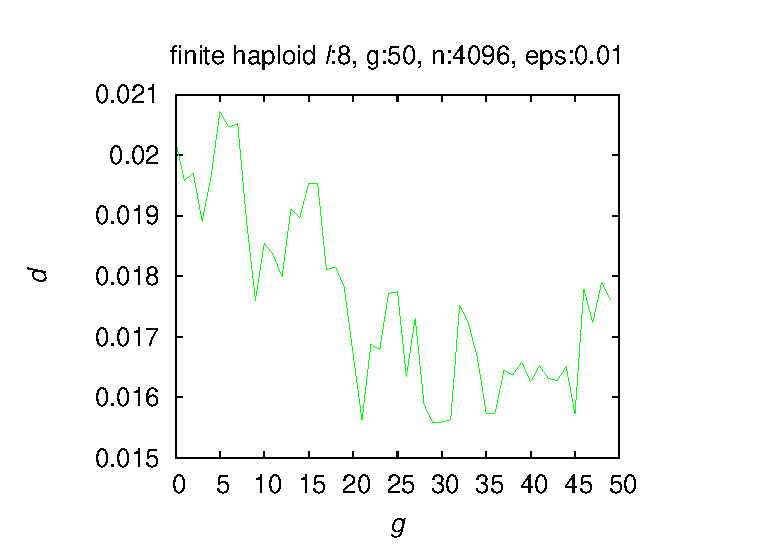
\includegraphics{figures/eps/vio/mu/b8/e0.01/n00004096_fin_hap.eps}}} \hspace{-3em}%
\subfloat{
\resizebox{8cm}{5cm}{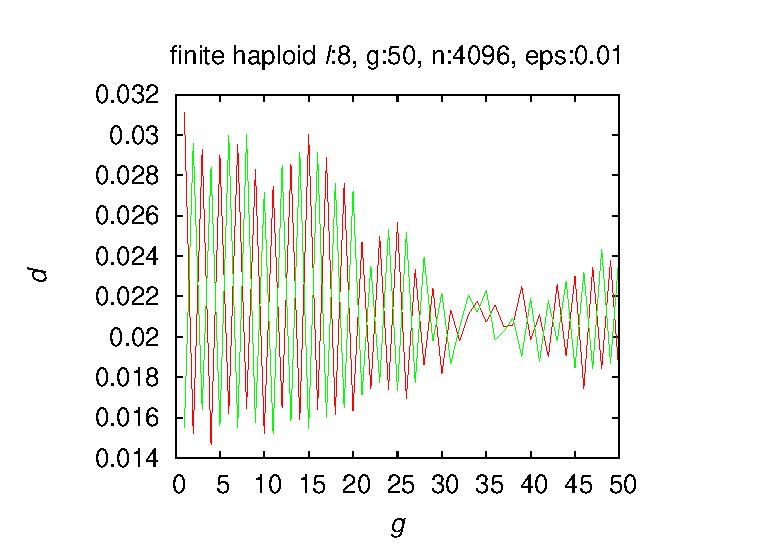
\includegraphics{figures/eps/vio/mu/b8/e0.01/n00004096_fin_hap_wovio.eps}}}\vspace{-1em} \hspace{-3em}%
\end{center}
\begin{center}
\subfloat{
\resizebox{8cm}{5cm}{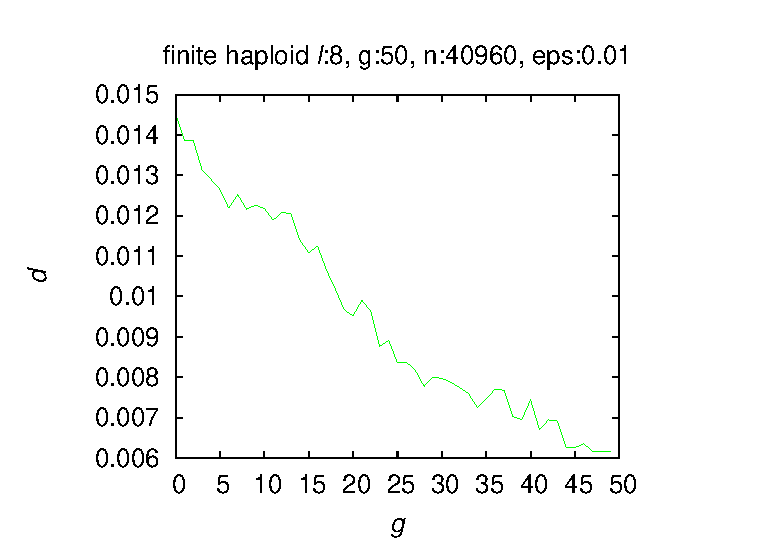
\includegraphics{figures/eps/vio/mu/b8/e0.01/n00040960_fin_hap.eps}}} \hspace{-3em}%
\subfloat{
\resizebox{8cm}{5cm}{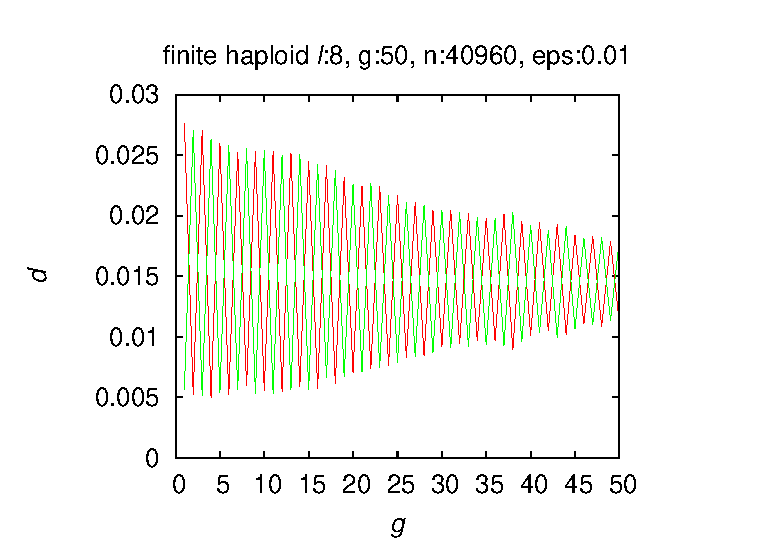
\includegraphics{figures/eps/vio/mu/b8/e0.01/n00040960_fin_hap_wovio.eps}}}\vspace{-1em} \hspace{-3em}%
\end{center}

\begin{center}
\subfloat{
\resizebox{8cm}{5cm}{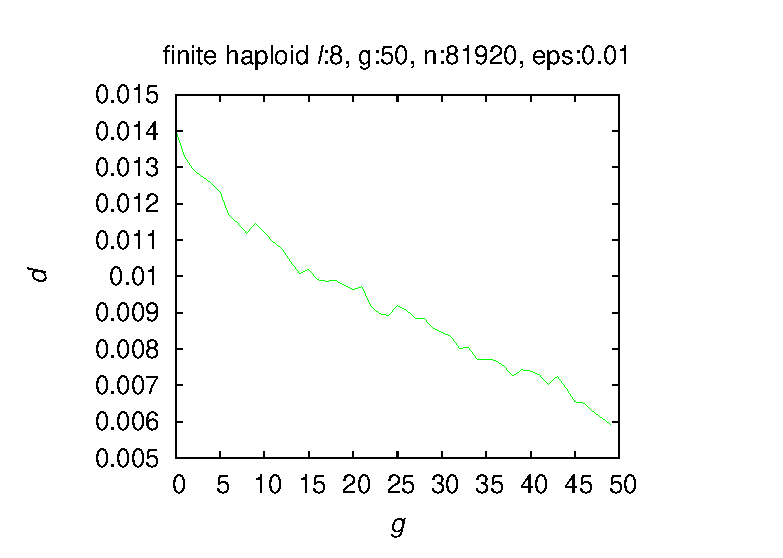
\includegraphics{figures/eps/vio/mu/b8/e0.01/n00081920_fin_hap.eps}}} \hspace{-3em}%
\subfloat{
\resizebox{8cm}{5cm}{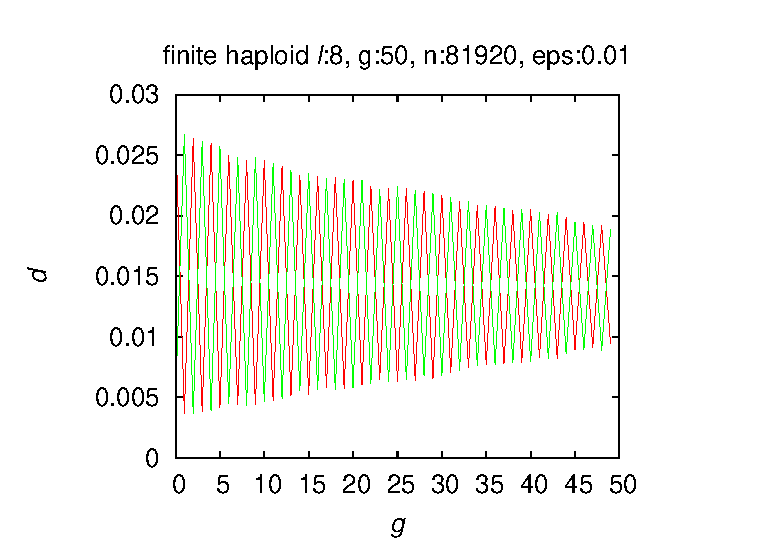
\includegraphics{figures/eps/vio/mu/b8/e0.01/n00081920_fin_hap_wovio.eps}}}\vspace{-1em} \hspace{-3em}%
\end{center}

\begin{center}
\subfloat{
\resizebox{8cm}{5cm}{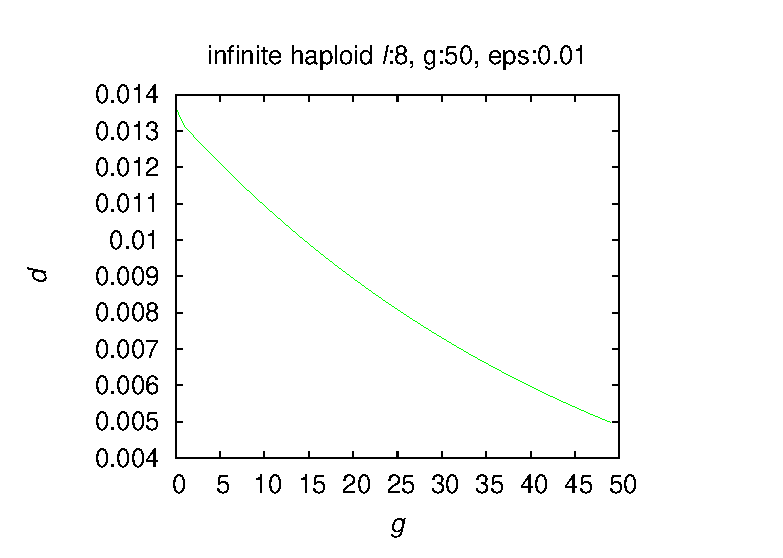
\includegraphics{figures/eps/vio/mu/b8/e0.01/inf_hap.eps}}}\hspace{-3em}%
\subfloat{
\resizebox{8cm}{5cm}{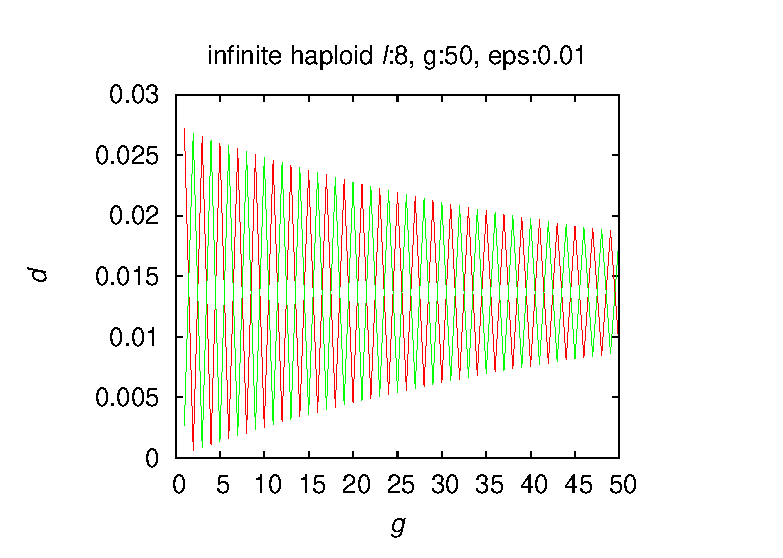
\includegraphics{figures/eps/vio/mu/b8/e0.01/inf_hap_wovio.eps}}}\vspace{-0.5em} \hspace{-3em}%
\caption{\textbf{Infinite and finite haploid population oscillation behavior in case of violation in $\bm{\mu}$ for genome length $\ell = 8$ and $\bm{\epsilon} = 0.01$:} 
  In left column, $d'$ is distance of finite population of size $n$ or infinite population to limit $\bm{z}^\ast$ for $g$ generations. In right column, $d$ is distance of finite population or infinite population to limits $\bm{p}^\ast$ and $\bm{q}^\ast$ without violation.}
\label{oscillation_8h_vio_mu_0.01}
\end{center}
\end{figure}

% l = 10

\begin{figure}[h]
\begin{center}
\subfloat{
\resizebox{8cm}{5cm}{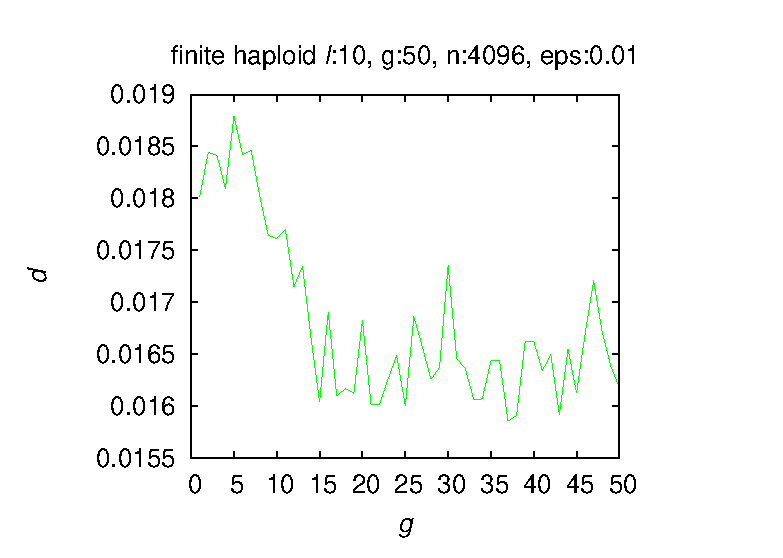
\includegraphics{figures/eps/vio/mu/b10/e0.01/n00004096_fin_hap.eps}}} \hspace{-3em}%
\subfloat{
\resizebox{8cm}{5cm}{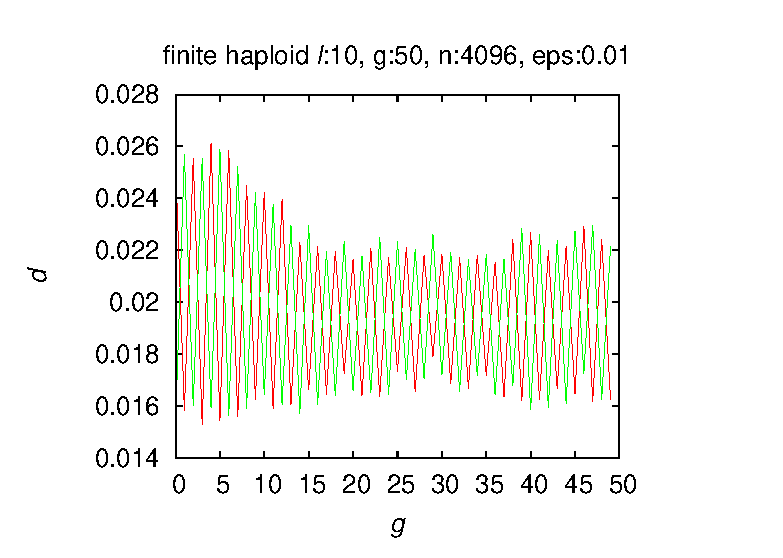
\includegraphics{figures/eps/vio/mu/b10/e0.01/n00004096_fin_hap_wovio.eps}}}\vspace{-1em} \hspace{-3em}%
\end{center}
\begin{center}
\subfloat{
\resizebox{8cm}{5cm}{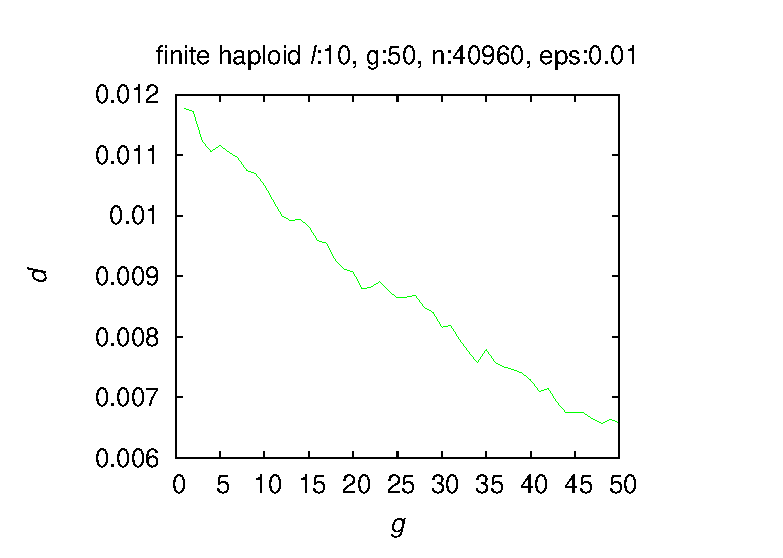
\includegraphics{figures/eps/vio/mu/b10/e0.01/n00040960_fin_hap.eps}}} \hspace{-3em}%
\subfloat{
\resizebox{8cm}{5cm}{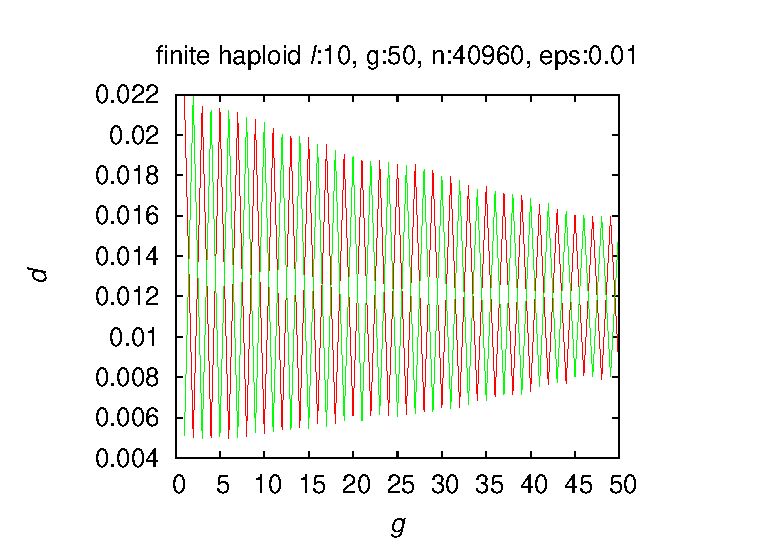
\includegraphics{figures/eps/vio/mu/b10/e0.01/n00040960_fin_hap_wovio.eps}}}\vspace{-1em} \hspace{-3em}%
\end{center}

\begin{center}
\subfloat{
\resizebox{8cm}{5cm}{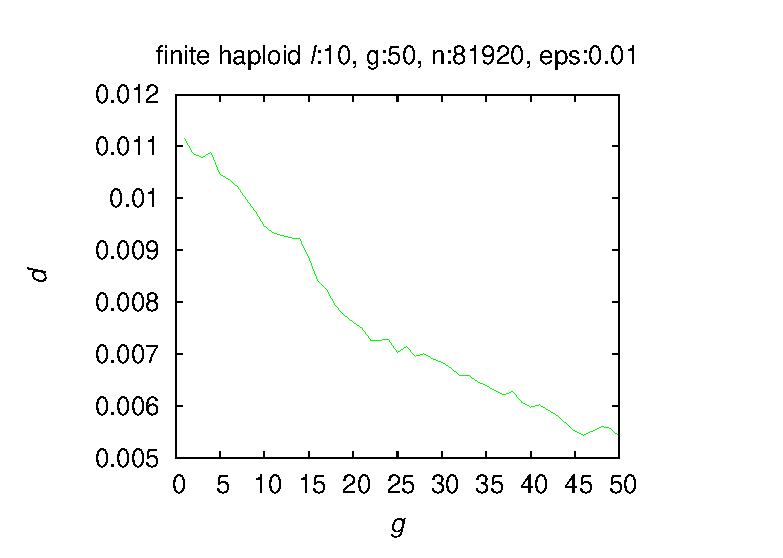
\includegraphics{figures/eps/vio/mu/b10/e0.01/n00081920_fin_hap.eps}}} \hspace{-3em}%
\subfloat{
\resizebox{8cm}{5cm}{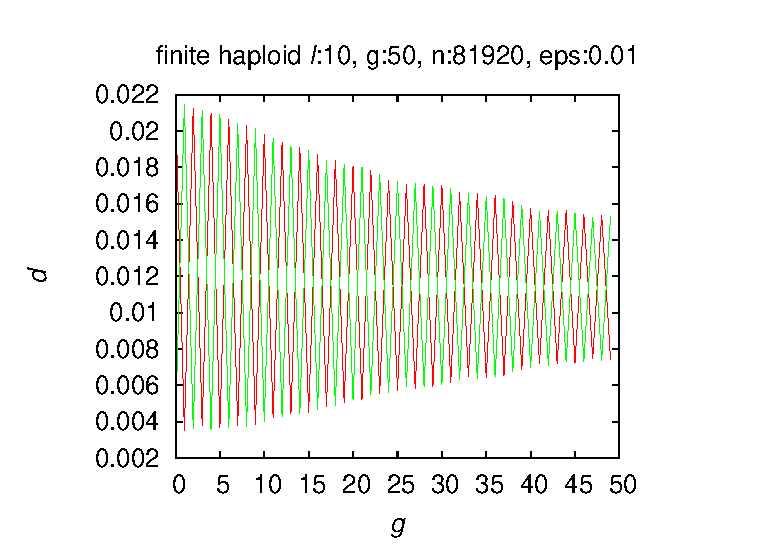
\includegraphics{figures/eps/vio/mu/b10/e0.01/n00081920_fin_hap_wovio.eps}}}\vspace{-1em} \hspace{-3em}%
\end{center}

\begin{center}
\subfloat{
\resizebox{8cm}{5cm}{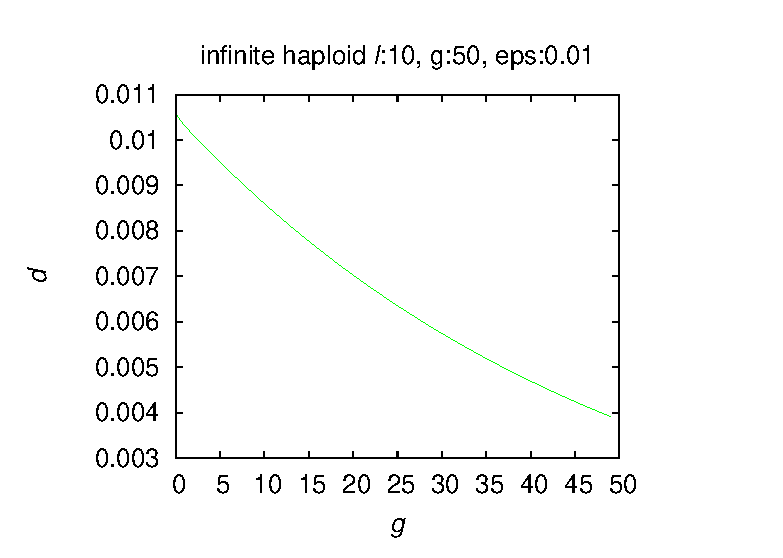
\includegraphics{figures/eps/vio/mu/b10/e0.01/inf_hap.eps}}}\hspace{-3em}%
\subfloat{
\resizebox{8cm}{5cm}{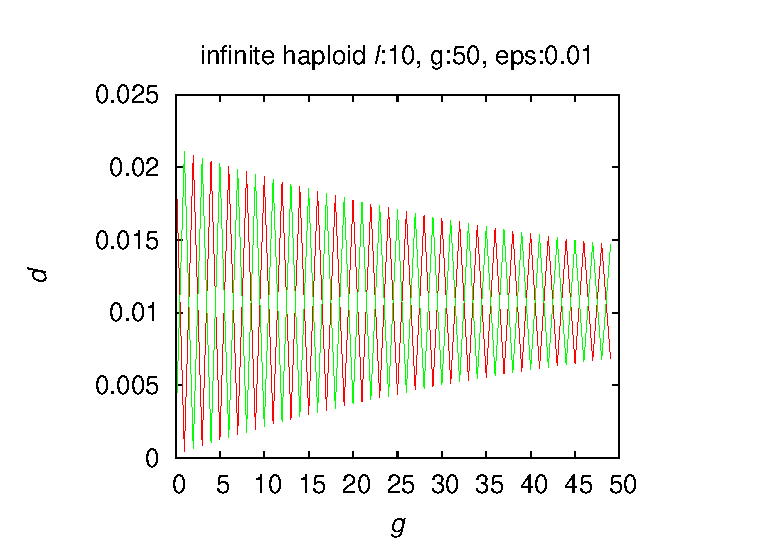
\includegraphics{figures/eps/vio/mu/b10/e0.01/inf_hap_wovio.eps}}}\vspace{-0.5em} \hspace{-3em}%
\caption{\textbf{Infinite and finite haploid population oscillation behavior in case of violation in $\bm{\mu}$ for genome length $\ell = 10$ and $\bm{\epsilon} = 0.01$:} 
  In left column, $d'$ is distance of finite population of size $n$ or infinite population to limit $\bm{z}^\ast$ for $g$ generations. In right column, $d$ is distance of finite population or infinite population to limits $\bm{p}^\ast$ and $\bm{q}^\ast$ without violation.}
\label{oscillation_10h_vio_mu_0.01}
\end{center}
\end{figure}

% l = 12

\begin{figure}[h]
\begin{center}
\subfloat{
\resizebox{8cm}{5cm}{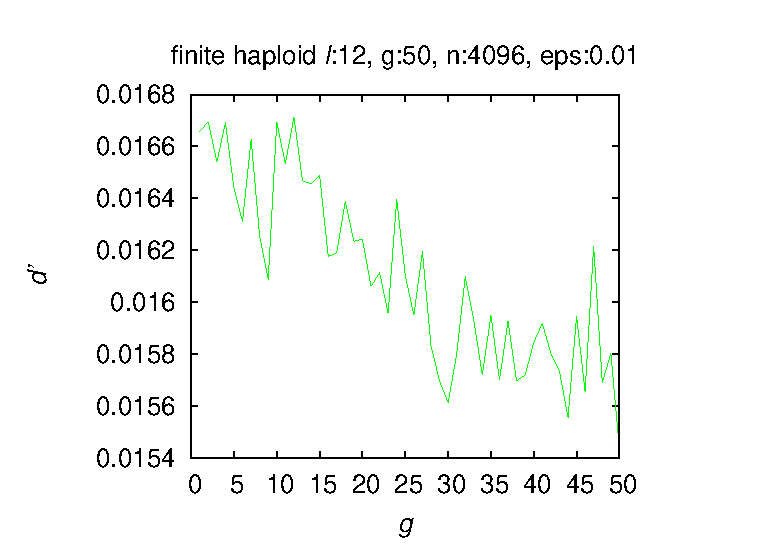
\includegraphics{figures/eps/vio/mu/b12/e0.01/n00004096_fin_hap.eps}}} \hspace{-3em}%
\subfloat{
\resizebox{8cm}{5cm}{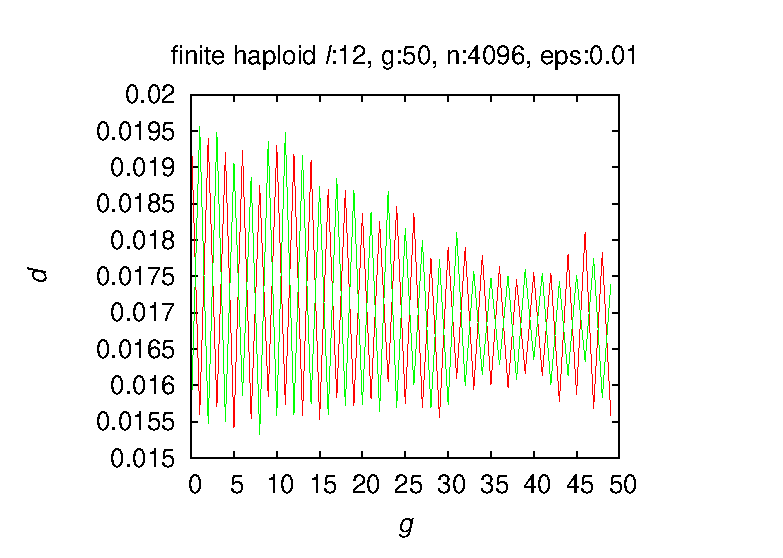
\includegraphics{figures/eps/vio/mu/b12/e0.01/n00004096_fin_hap_wovio.eps}}}\vspace{-1em} \hspace{-3em}%
\end{center}
\begin{center}
\subfloat{
\resizebox{8cm}{5cm}{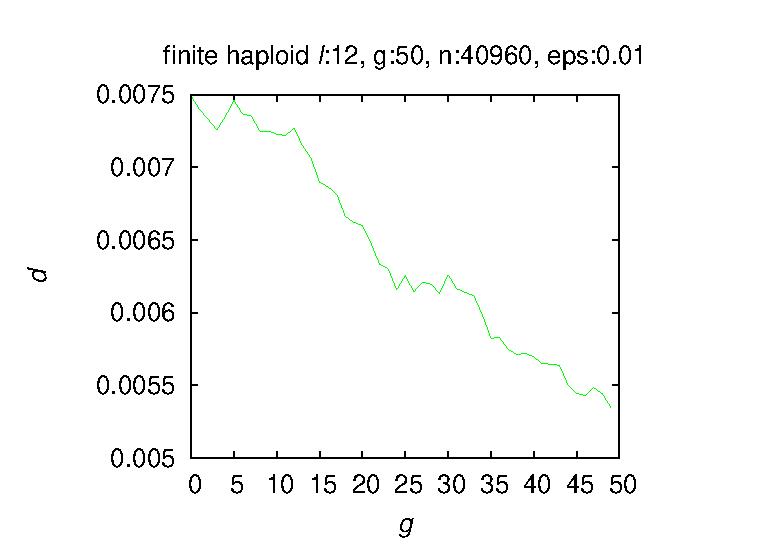
\includegraphics{figures/eps/vio/mu/b12/e0.01/n00040960_fin_hap.eps}}} \hspace{-3em}%
\subfloat{
\resizebox{8cm}{5cm}{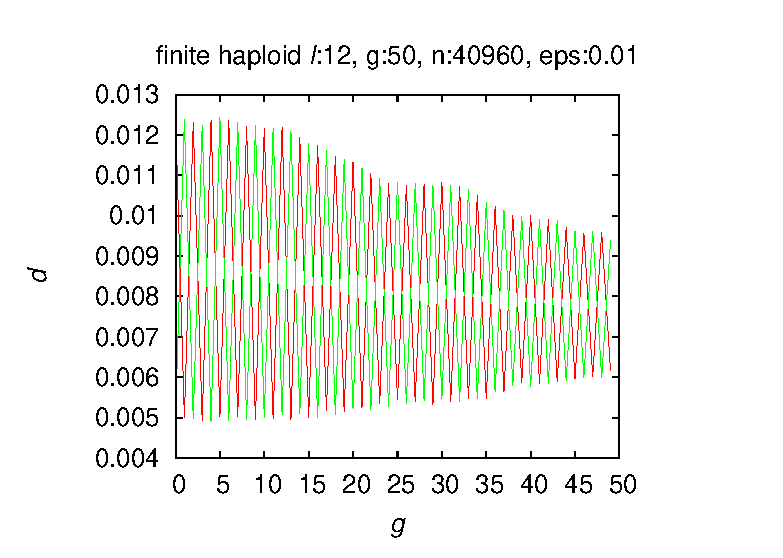
\includegraphics{figures/eps/vio/mu/b12/e0.01/n00040960_fin_hap_wovio.eps}}}\vspace{-1em} \hspace{-3em}%
\end{center}

\begin{center}
\subfloat{
\resizebox{8cm}{5cm}{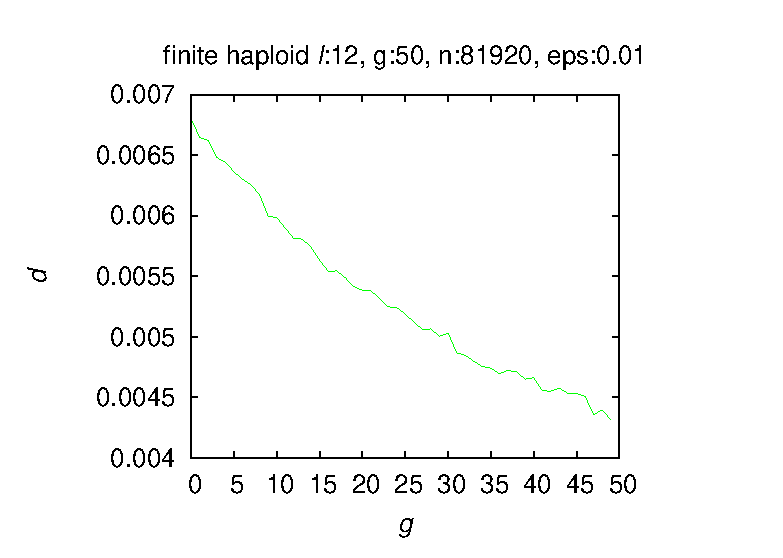
\includegraphics{figures/eps/vio/mu/b12/e0.01/n00081920_fin_hap.eps}}} \hspace{-3em}%
\subfloat{
\resizebox{8cm}{5cm}{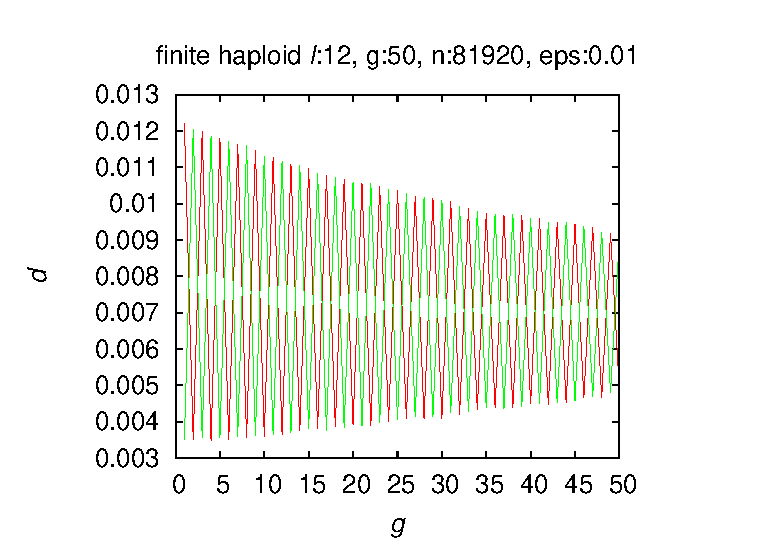
\includegraphics{figures/eps/vio/mu/b12/e0.01/n00081920_fin_hap_wovio.eps}}}\vspace{-1em} \hspace{-3em}%
\end{center}

\begin{center}
\subfloat{
\resizebox{8cm}{5cm}{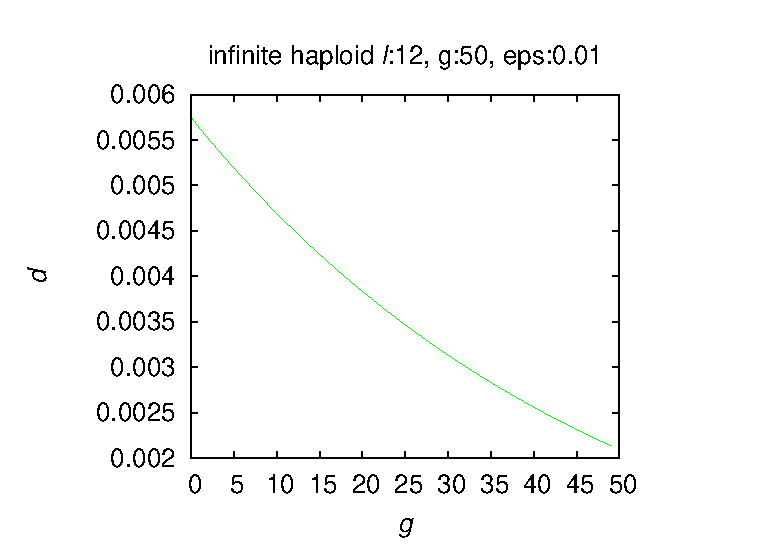
\includegraphics{figures/eps/vio/mu/b12/e0.01/inf_hap.eps}}}\hspace{-3em}%
\subfloat{
\resizebox{8cm}{5cm}{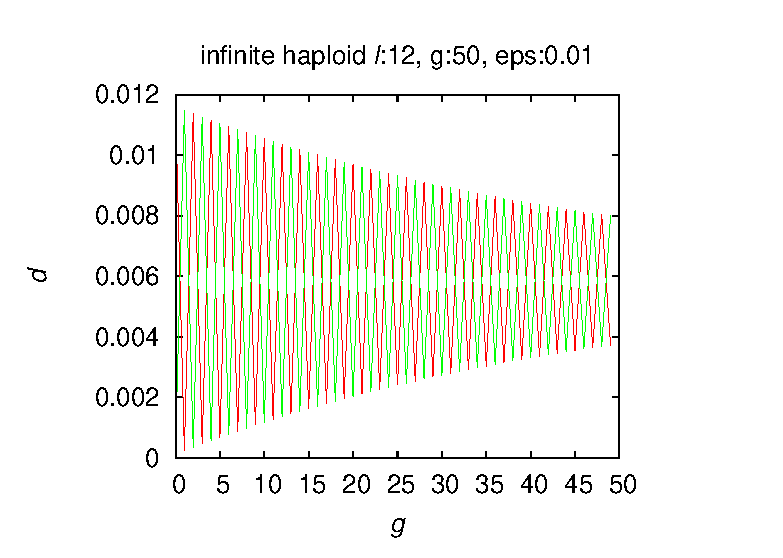
\includegraphics{figures/eps/vio/mu/b12/e0.01/inf_hap_wovio.eps}}}\vspace{-0.5em} \hspace{-3em}%
\caption{\textbf{Infinite and finite haploid population oscillation behavior in case of violation in $\bm{\mu}$ for genome length $\ell = 12$ and $\bm{\epsilon} = 0.01$:} 
  In left column, $d'$ is distance of finite population of size $n$ or infinite population to limit $\bm{z}^\ast$ for $g$ generations. In right column, $d$ is distance of finite population or infinite population to limits $\bm{p}^\ast$ and $\bm{q}^\ast$ without violation.}
\label{oscillation_12h_vio_mu_0.01}
\end{center}
\end{figure}

% l = 14

\begin{figure}[h]
\begin{center}
\subfloat{
\resizebox{8cm}{5cm}{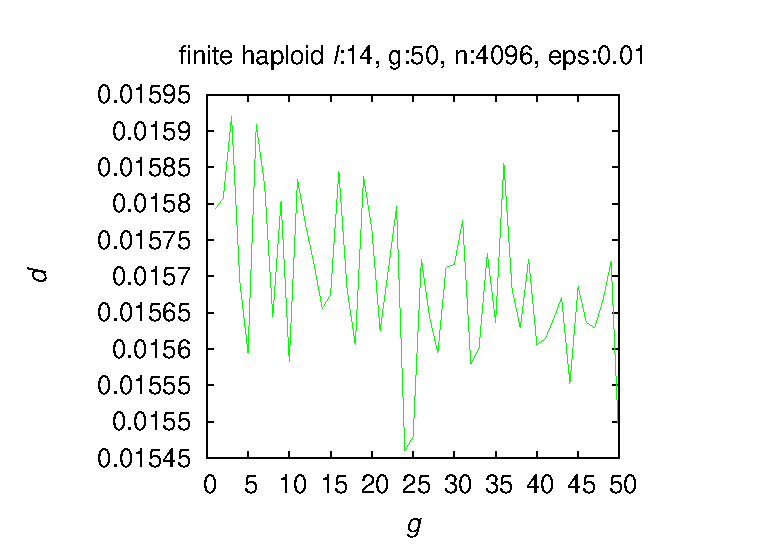
\includegraphics{figures/eps/vio/mu/b14/e0.01/n00004096_fin_hap.eps}}} \hspace{-3em}%
\subfloat{
\resizebox{8cm}{5cm}{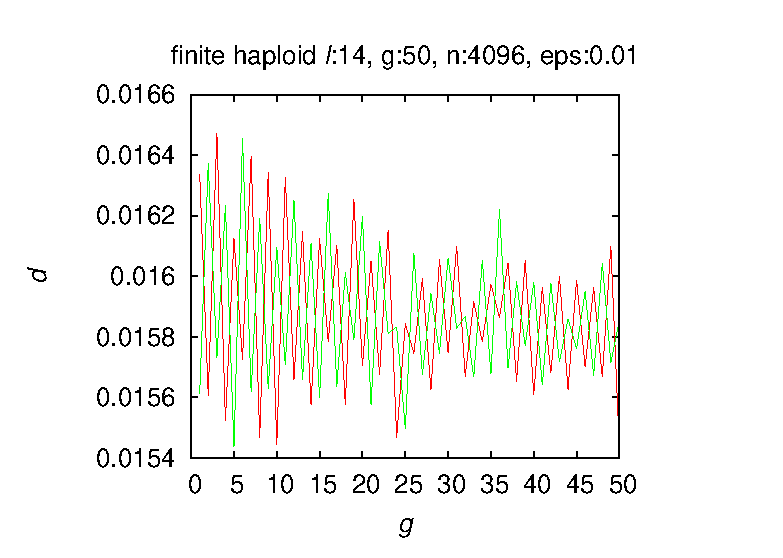
\includegraphics{figures/eps/vio/mu/b14/e0.01/n00004096_fin_hap_wovio.eps}}}\vspace{-1em} \hspace{-3em}%
\end{center}
\begin{center}
\subfloat{
\resizebox{8cm}{5cm}{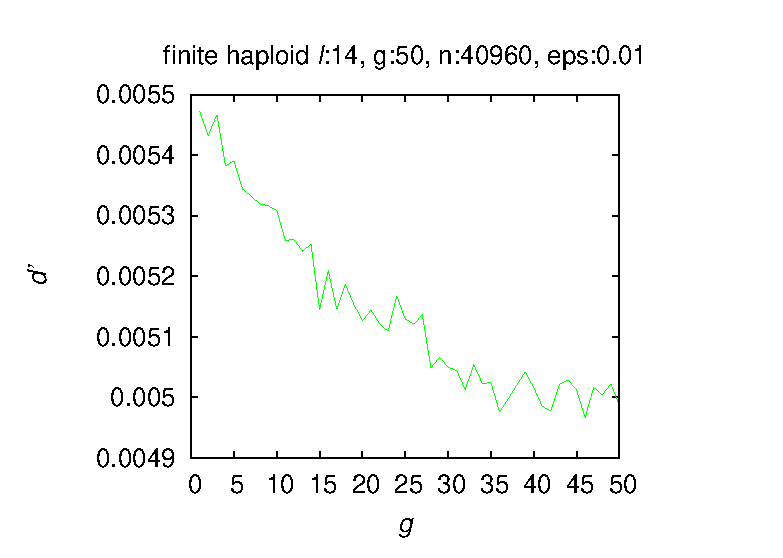
\includegraphics{figures/eps/vio/mu/b14/e0.01/n00040960_fin_hap.eps}}} \hspace{-3em}%
\subfloat{
\resizebox{8cm}{5cm}{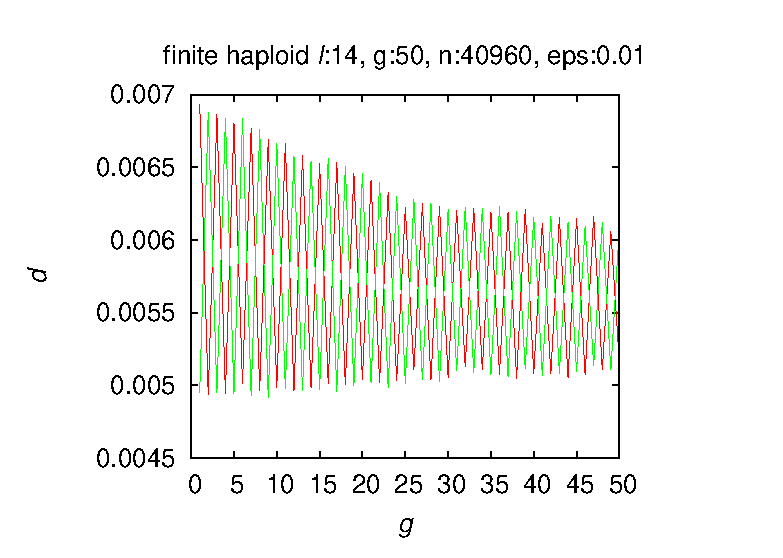
\includegraphics{figures/eps/vio/mu/b14/e0.01/n00040960_fin_hap_wovio.eps}}}\vspace{-1em} \hspace{-3em}%
\end{center}

\begin{center}
\subfloat{
\resizebox{8cm}{5cm}{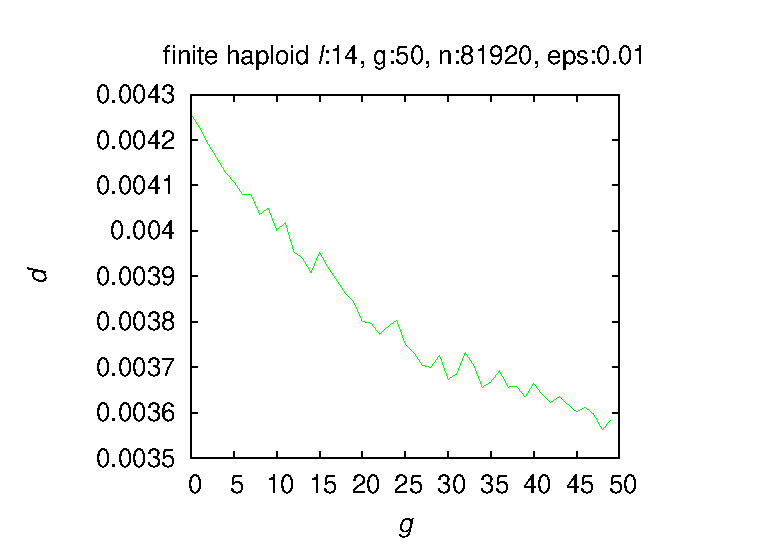
\includegraphics{figures/eps/vio/mu/b14/e0.01/n00081920_fin_hap.eps}}} \hspace{-3em}%
\subfloat{
\resizebox{8cm}{5cm}{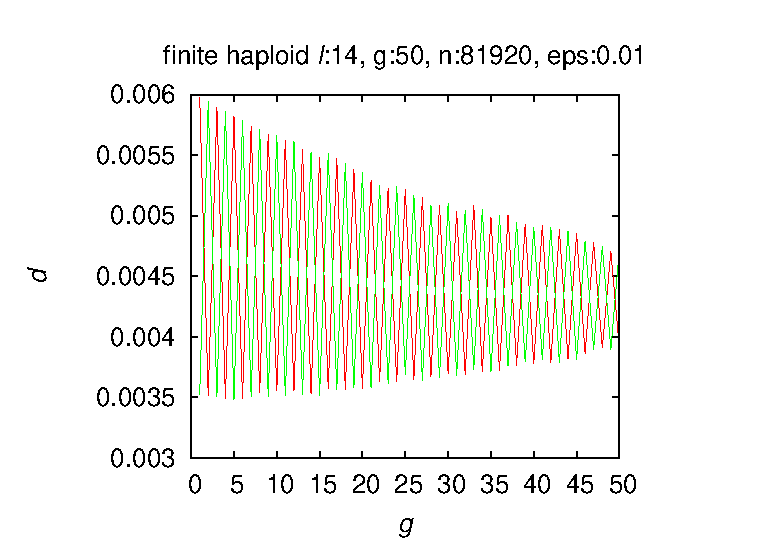
\includegraphics{figures/eps/vio/mu/b14/e0.01/n00081920_fin_hap_wovio.eps}}}\vspace{-1em} \hspace{-3em}%
\end{center}

\begin{center}
\subfloat{
\resizebox{8cm}{5cm}{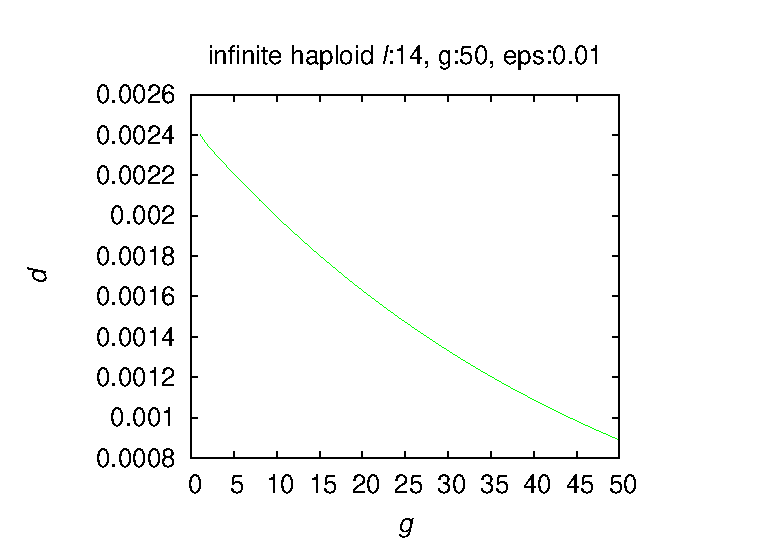
\includegraphics{figures/eps/vio/mu/b14/e0.01/inf_hap.eps}}}\hspace{-3em}%
\subfloat{
\resizebox{8cm}{5cm}{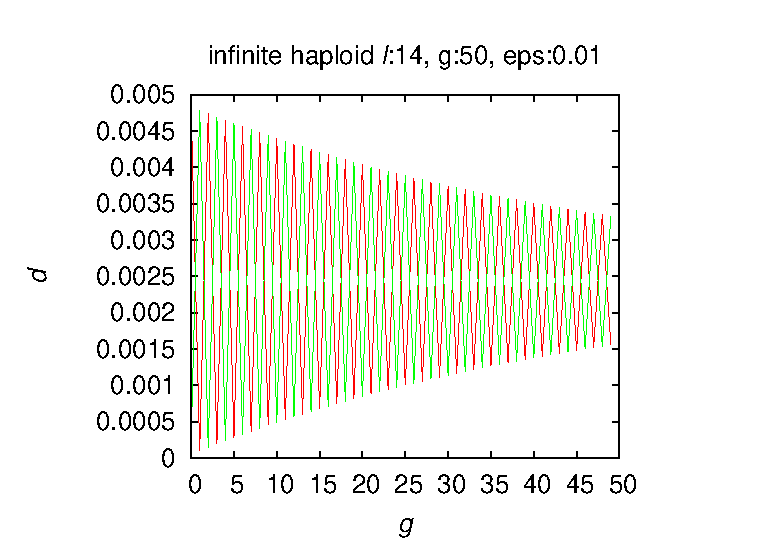
\includegraphics{figures/eps/vio/mu/b14/e0.01/inf_hap_wovio.eps}}}\vspace{-0.5em} \hspace{-3em}%
\caption{\textbf{Infinite and finite haploid population oscillation behavior in case of violation in $\bm{\mu}$ for genome length $\ell = 14$ and $\bm{\epsilon} = 0.01$:} 
  In left column, $d'$ is distance of finite population of size $n$ or infinite population to limit $\bm{z}^\ast$ for $g$ generations. In right column, $d$ is distance of finite population or infinite population to limits $\bm{p}^\ast$ and $\bm{q}^\ast$ without violation.}
\label{oscillation_14h_vio_mu_0.01}
\end{center}
\end{figure}

\clearpage

The right column in figures \ref{oscillation_8h_vio_mu_0.01} through \ref{oscillation_14h_vio_mu_0.01} 
shows distance of finite and infinite haploid populations to non-violation limits $\bm{p^\ast}$ and $\bm{q^\ast}$ with $\bm{\epsilon} \;=\; 0.01$. 
Those graphs indicate oscillating behavior of haploid population given violation. 
Both finite and infinite populations oscillate given violation. Oscillations are sharper. Since the value of $\bm{\epsilon}$ 
is small, damping of ripples is slow. The all zeros mask created in mutation distribution with $\bm{\epsilon} \;=\; 0.01$ have small 
probability of being used during mutation, and when it is not used, behavior should be consistent with the 
behavior without violation. Moreover, $\bm{\epsilon}$ is so small that 
infinite population oscillation does not die out completely in 50 generations.

The left column of figures \ref{oscillation_8h_vio_mu_0.01} through \ref{oscillation_14h_vio_mu_0.01} 
shows distance of finite and infinite haploid populations to limit $\bm{z^\ast}$ 
(limit with violation in mutation distribution $\bm{\mu}$) when $\bm{\epsilon} \;=\; 0.01$. 
The distance between finite population and limit $\bm{z}^\ast$ (limit with violation in $\bm{\mu}$ distribution) 
decreases as finite population size increases, 
and finite population shows behavior similar to infinite population behavior as finite population reach large number. 
Average distance data for haploid population in case of violation in $\bm{\mu}$ distribution 
with $\bm{\epsilon} \;=\; 0.01$ for different finite population size $N$ are tabulated in table \ref{distanceMuHapEps0.01}.

\begin{table}[ht]
\caption{\textbf{Distance measured for violation in $\bm{\mu}$ with $\bm{\epsilon} \;=\; 0.01$ for haploids:} $\ell$ is genome length, 
average distance between finite and infinite population is tabulated in the last three columns, and last row is expected single step distance.}
\centering
\begin{tabularx}{0.75\textwidth}{ c *{3}{X}}
\toprule
$\ell$ & $N = 4096$ & $N = 40960$ & $N = 81920$ \\
\midrule
8 & 0.0176	& 0.0094	& 0.0093 \\
10 & 0.0168	& 0.0088 	& 0.0077 \\ 
12 & 0.0161	& 0.0064 	& 0.0053 \\
14 & 0.0157	& 0.0051 	& 0.0038 \\ 
\midrule
$1/\sqrt{N}$ & 0.0156 & 0.0049 & 0.0035 \\
\bottomrule
\end{tabularx}
\label{distanceMuHapEps0.01}
\end{table}

From table \ref{distanceMuHapEps0.01}, average distance calculated for finite population size $4096$ is $0.0165$, 
for size $40960$ is $0.0074$ and for size $81920$ is $0.0065$. These results show average distance 
between finite population and limit $\bm{z^\ast}$ approach the expected single step distance 
between finite and infinite population. The distance decreased as $1/\sqrt{N}$. 
Also, the distance decreased as genome length $\ell$ increased for all sizes of finite haploid populations 
with $\bm{\epsilon} \;=\; 0.01$.


\subsection{Haploid Population $\mathtt{\sim}$ $\epsilon: 0.1$}
% l = 8

\begin{figure}[h]
\begin{center}
\subfloat{
\resizebox{8cm}{5cm}{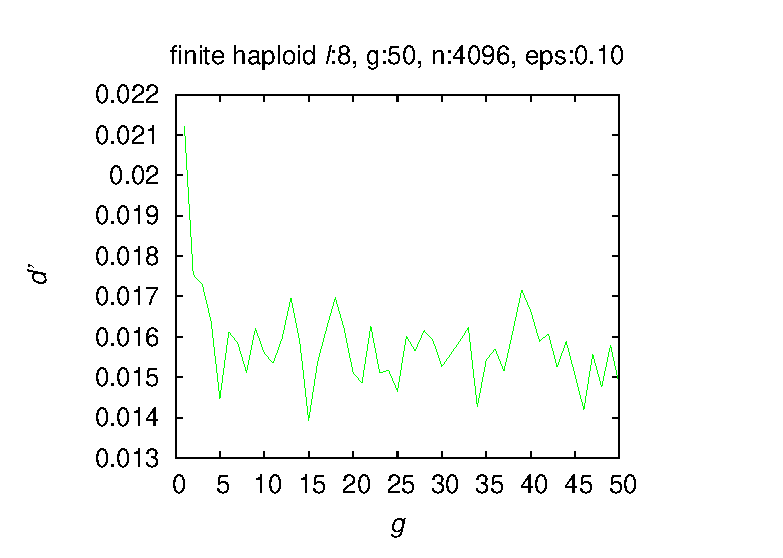
\includegraphics{figures/eps/vio/mu/b8/e0.1/n00004096_fin_hap.eps}}} \hspace{-3em}%
\subfloat{
\resizebox{8cm}{5cm}{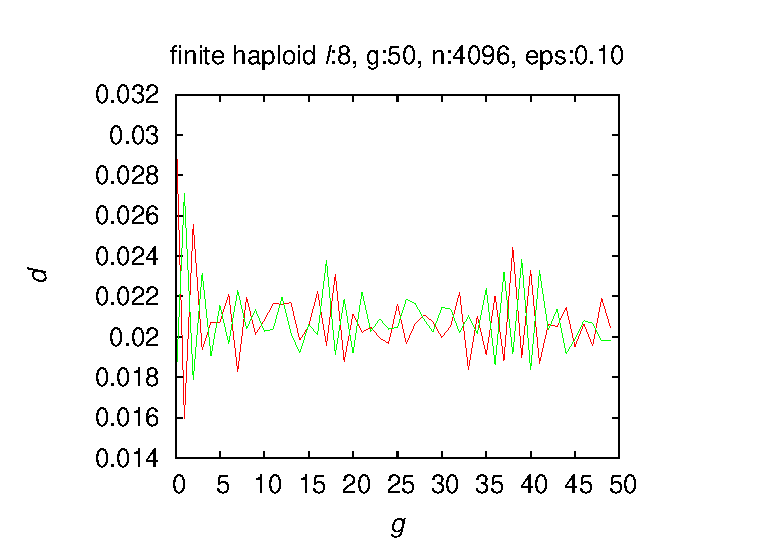
\includegraphics{figures/eps/vio/mu/b8/e0.1/n00004096_fin_hap_wovio.eps}}}\vspace{-1em} \hspace{-3em}%
\end{center}
\begin{center}
\subfloat{
\resizebox{8cm}{5cm}{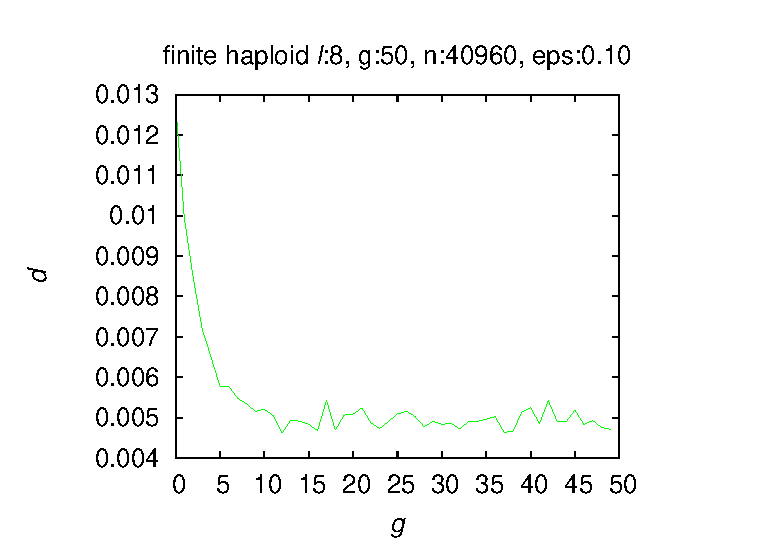
\includegraphics{figures/eps/vio/mu/b8/e0.1/n00040960_fin_hap.eps}}} \hspace{-3em}%
\subfloat{
\resizebox{8cm}{5cm}{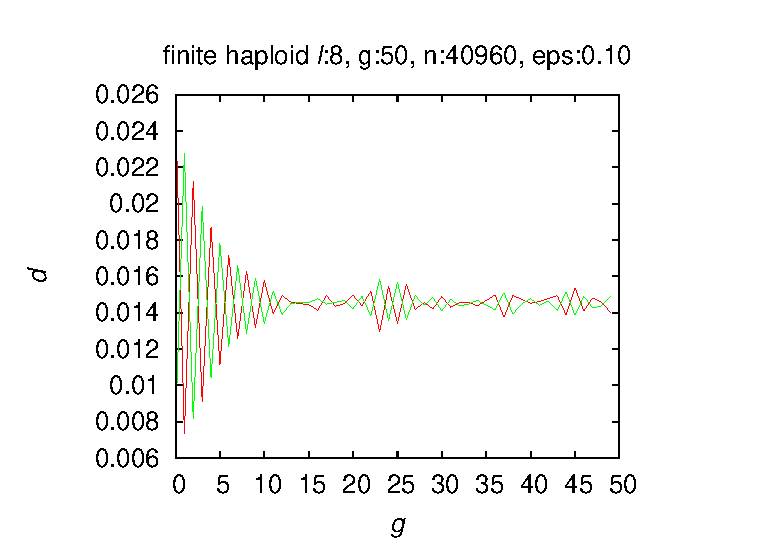
\includegraphics{figures/eps/vio/mu/b8/e0.1/n00040960_fin_hap_wovio.eps}}}\vspace{-1em} \hspace{-3em}%
\end{center}

\begin{center}
\subfloat{
\resizebox{8cm}{5cm}{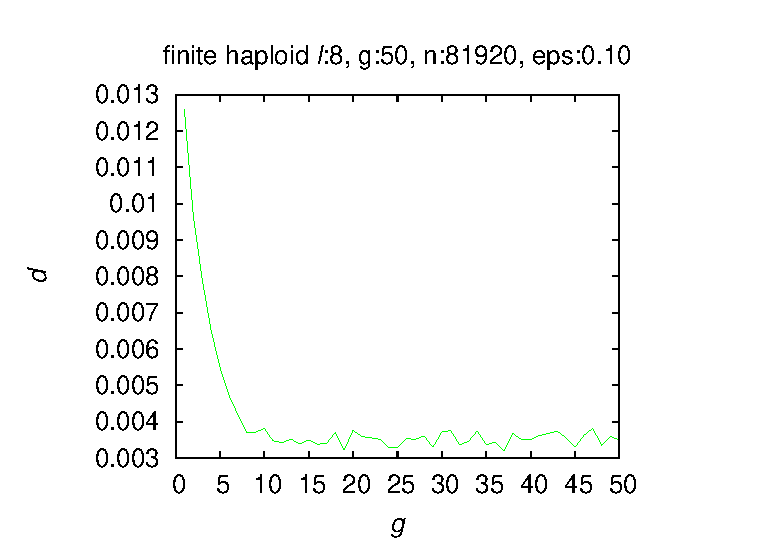
\includegraphics{figures/eps/vio/mu/b8/e0.1/n00081920_fin_hap.eps}}} \hspace{-3em}%
\subfloat{
\resizebox{8cm}{5cm}{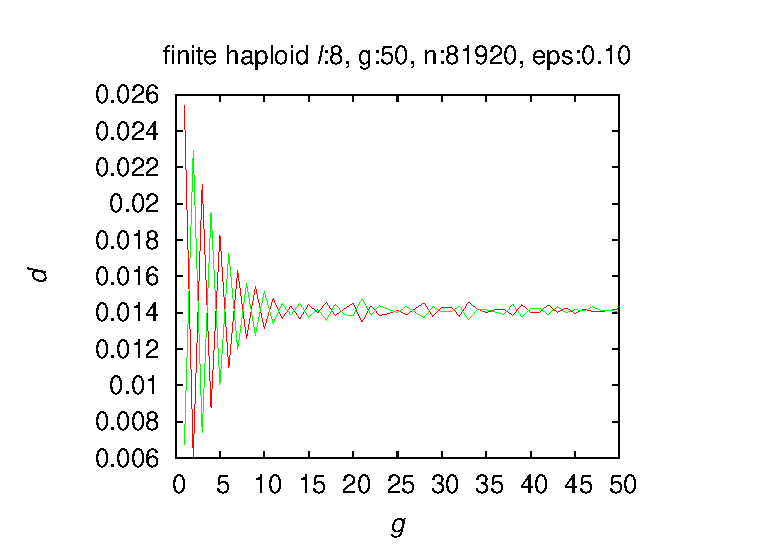
\includegraphics{figures/eps/vio/mu/b8/e0.1/n00081920_fin_hap_wovio.eps}}}\vspace{-1em} \hspace{-3em}%
\end{center}

\begin{center}
\subfloat{
\resizebox{8cm}{5cm}{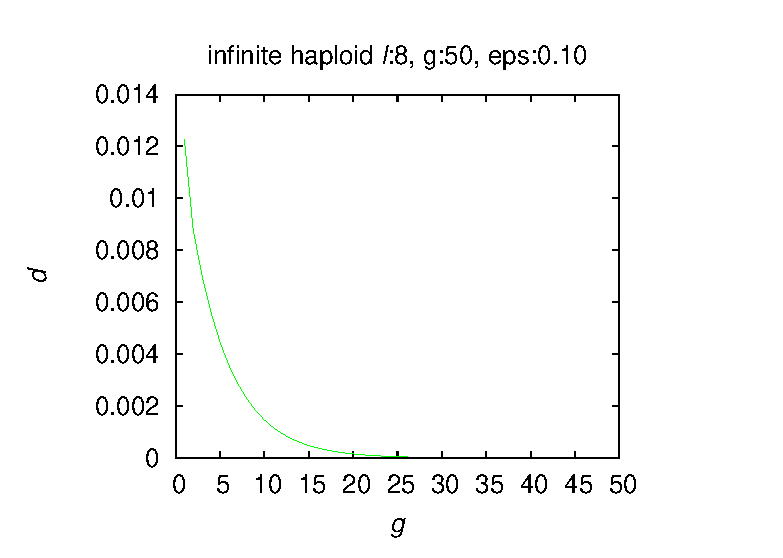
\includegraphics{figures/eps/vio/mu/b8/e0.1/inf_hap.eps}}}\hspace{-3em}%
\subfloat{
\resizebox{8cm}{5cm}{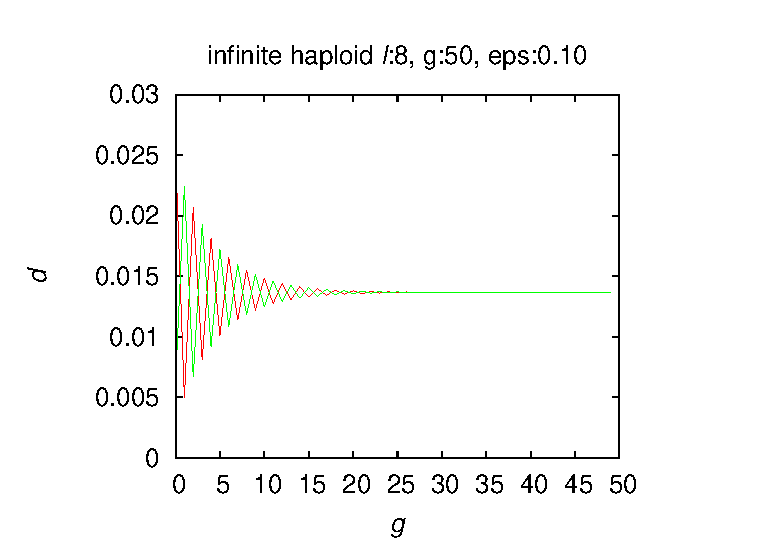
\includegraphics{figures/eps/vio/mu/b8/e0.1/inf_hap_wovio.eps}}}\vspace{-0.5em} \hspace{-3em}%


\caption[\textbf{Infinite and finite haploid population oscillation behavior in case of violation in $\bm{\mu}$ for genome length $\ell = 8$ and $\bm{\epsilon} = 0.1$}]{\textbf{Infinite and finite haploid population oscillation behavior in case of violation in $\bm{\mu}$ for genome length $\ell = 8$ and $\bm{\epsilon} = 0.1$:} 
  In left column, $d'$ is distance of finite population of size $n$ or infinite population to limit $\bm{z}^\ast$ for $g$ generations. In right column, $d$ is distance of finite population or infinite population to limits $\bm{p}^\ast$ and $\bm{q}^\ast$ without violation.}
\label{oscillation_8h_vio_mu_0.1}
\end{center}
\end{figure}

% l = 10

\begin{figure}[h]
\begin{center}
\subfloat{
\resizebox{8cm}{5cm}{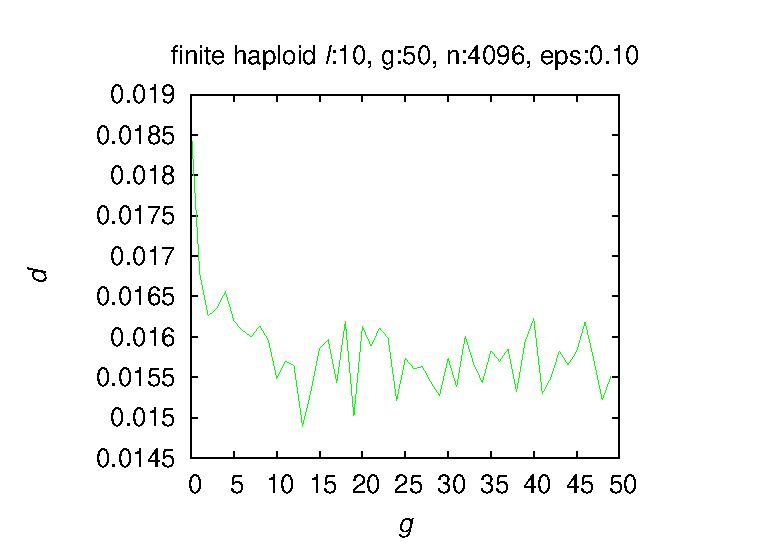
\includegraphics{figures/eps/vio/mu/b10/e0.1/n00004096_fin_hap.eps}}} \hspace{-3em}%
\subfloat{
\resizebox{8cm}{5cm}{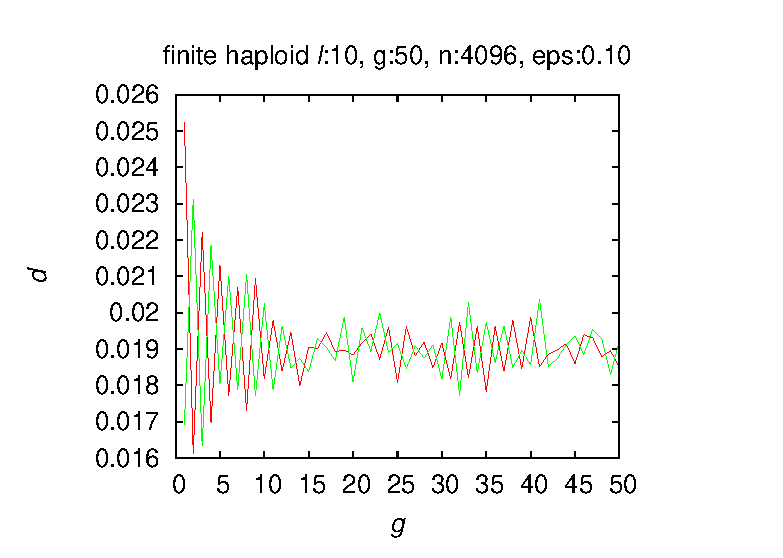
\includegraphics{figures/eps/vio/mu/b10/e0.1/n00004096_fin_hap_wovio.eps}}}\vspace{-1em} \hspace{-3em}%
\end{center}
\begin{center}
\subfloat{
\resizebox{8cm}{5cm}{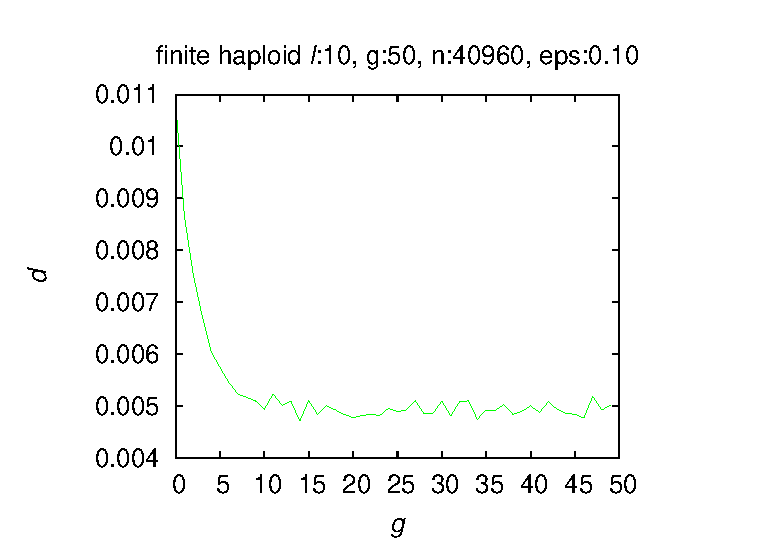
\includegraphics{figures/eps/vio/mu/b10/e0.1/n00040960_fin_hap.eps}}} \hspace{-3em}%
\subfloat{
\resizebox{8cm}{5cm}{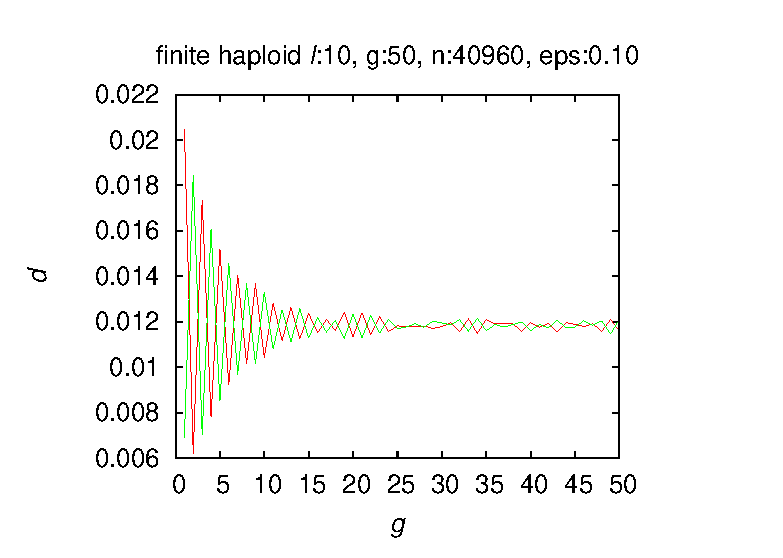
\includegraphics{figures/eps/vio/mu/b10/e0.1/n00040960_fin_hap_wovio.eps}}}\vspace{-1em} \hspace{-3em}%
\end{center}

\begin{center}
\subfloat{
\resizebox{8cm}{5cm}{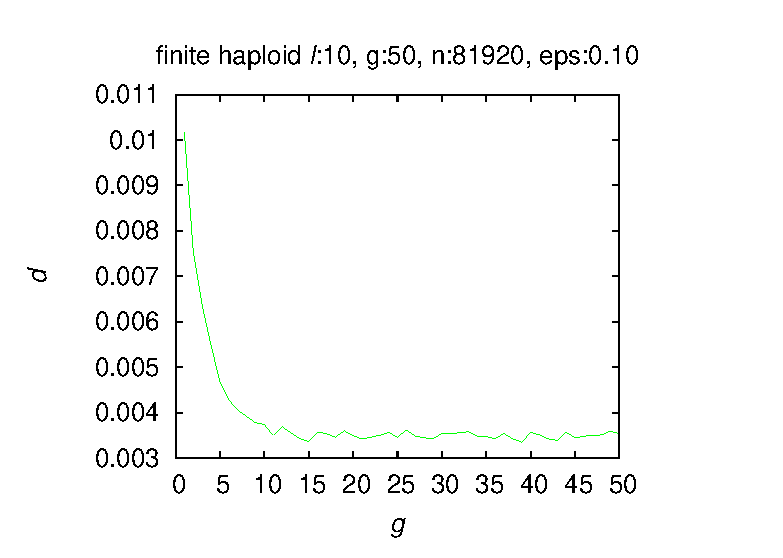
\includegraphics{figures/eps/vio/mu/b10/e0.1/n00081920_fin_hap.eps}}} \hspace{-3em}%
\subfloat{
\resizebox{8cm}{5cm}{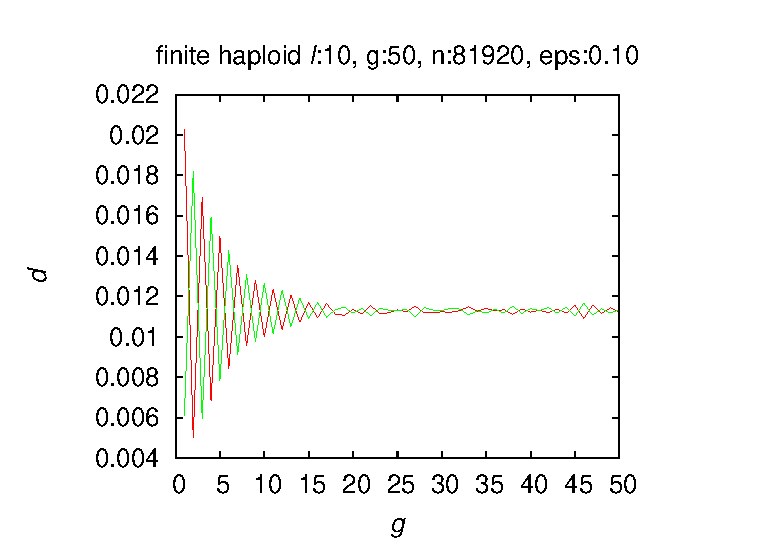
\includegraphics{figures/eps/vio/mu/b10/e0.1/n00081920_fin_hap_wovio.eps}}}\vspace{-1em} \hspace{-3em}%
\end{center}

\begin{center}
\subfloat{
\resizebox{8cm}{5cm}{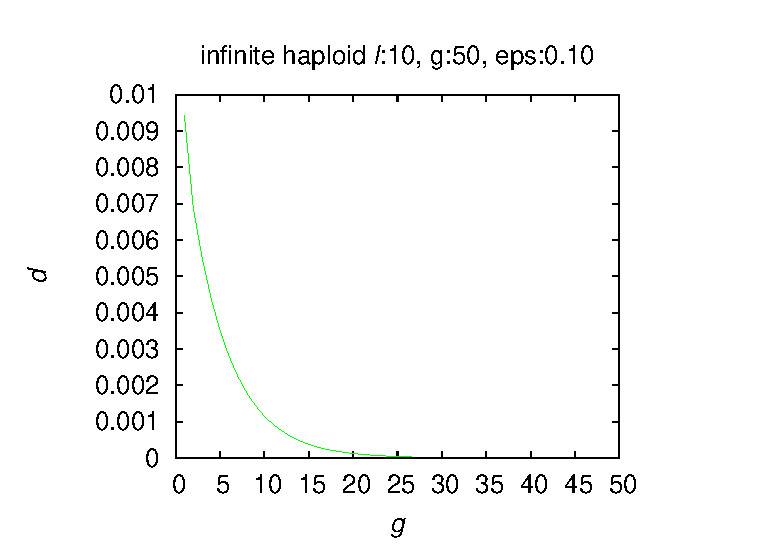
\includegraphics{figures/eps/vio/mu/b10/e0.1/inf_hap.eps}}}\hspace{-3em}%
\subfloat{
\resizebox{8cm}{5cm}{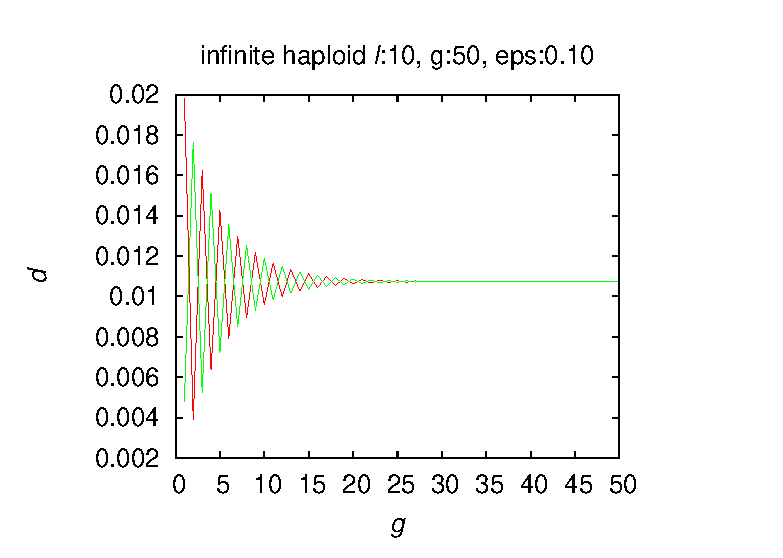
\includegraphics{figures/eps/vio/mu/b10/e0.1/inf_hap_wovio.eps}}}\vspace{-0.5em} \hspace{-3em}%


\caption[\textbf{Infinite and finite haploid population oscillation behavior in case of violation in $\bm{\mu}$ for genome length $\ell = 10$ and $\bm{\epsilon} = 0.1$}]{\textbf{Infinite and finite haploid population oscillation behavior in case of violation in $\bm{\mu}$ for genome length $\ell = 10$ and $\bm{\epsilon} = 0.1$:} 
  In left column, $d'$ is distance of finite population of size $n$ or infinite population to limit $\bm{z}^\ast$ for $g$ generations. In right column, $d$ is distance of finite population or infinite population to limits $\bm{p}^\ast$ and $\bm{q}^\ast$ without violation.}
\label{oscillation_10h_vio_mu_0.1}
\end{center}
\end{figure}

% l = 12

\begin{figure}[h]
\begin{center}
\subfloat{
\resizebox{8cm}{5cm}{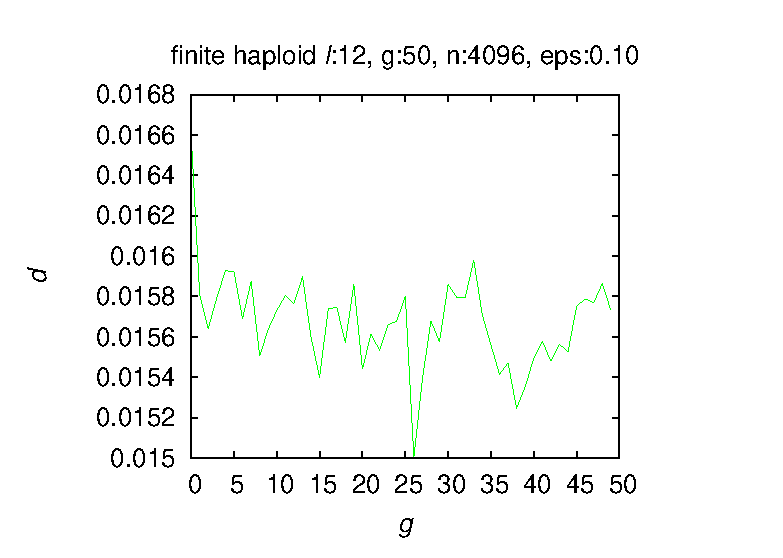
\includegraphics{figures/eps/vio/mu/b12/e0.1/n00004096_fin_hap.eps}}} \hspace{-3em}%
\subfloat{
\resizebox{8cm}{5cm}{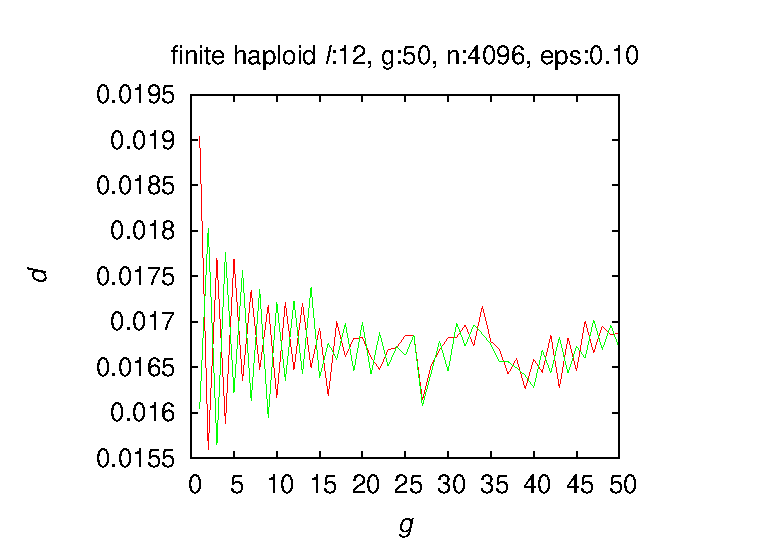
\includegraphics{figures/eps/vio/mu/b12/e0.1/n00004096_fin_hap_wovio.eps}}}\vspace{-1em} \hspace{-3em}%
\end{center}
\begin{center}
\subfloat{
\resizebox{8cm}{5cm}{\includegraphics{figures/eps/vio/mu/b12/e0.1/n00040960_fin_hap.eps}}} \hspace{-3em}%
\subfloat{
\resizebox{8cm}{5cm}{\includegraphics{figures/eps/vio/mu/b12/e0.1/n00040960_fin_hap_wovio.eps}}}\vspace{-1em} \hspace{-3em}%
\end{center}

\begin{center}
\subfloat{
\resizebox{8cm}{5cm}{\includegraphics{figures/eps/vio/mu/b12/e0.1/n00081920_fin_hap.eps}}} \hspace{-3em}%
\subfloat{
\resizebox{8cm}{5cm}{\includegraphics{figures/eps/vio/mu/b12/e0.1/n00081920_fin_hap_wovio.eps}}}\vspace{-1em} \hspace{-3em}%
\end{center}

\begin{center}
\subfloat{
\resizebox{8cm}{5cm}{\includegraphics{figures/eps/vio/mu/b12/e0.1/inf_hap.eps}}}\hspace{-3em}%
\subfloat{
\resizebox{8cm}{5cm}{\includegraphics{figures/eps/vio/mu/b12/e0.1/inf_hap_wovio.eps}}}\vspace{-0.5em} \hspace{-3em}%


\caption[\textbf{Infinite and finite haploid population oscillation behavior in case of violation in $\bm{\mu}$ for genome length $\ell = 12$ and $\bm{\epsilon} = 0.1$}]{\textbf{Infinite and finite haploid population oscillation behavior in case of violation in $\bm{\mu}$ for genome length $\ell = 12$ and $\bm{\epsilon} = 0.1$:} 
  In left column, $d'$ is distance of finite population of size $n$ or infinite population to limit $\bm{z}^\ast$ for $g$ generations. In right column, $d$ is distance of finite population or infinite population to limits $\bm{p}^\ast$ and $\bm{q}^\ast$ without violation.}
\label{oscillation_12h_vio_mu_0.1}
\end{center}
\end{figure}

% l = 14

\begin{figure}[h]
\begin{center}
\subfloat{
\resizebox{8cm}{5cm}{\includegraphics{figures/eps/vio/mu/b14/e0.1/n00004096_fin_hap.eps}}} \hspace{-3em}%
\subfloat{
\resizebox{8cm}{5cm}{\includegraphics{figures/eps/vio/mu/b14/e0.1/n00004096_fin_hap_wovio.eps}}}\vspace{-1em} \hspace{-3em}%
\end{center}
\begin{center}
\subfloat{
\resizebox{8cm}{5cm}{\includegraphics{figures/eps/vio/mu/b14/e0.1/n00040960_fin_hap.eps}}} \hspace{-3em}%
\subfloat{
\resizebox{8cm}{5cm}{\includegraphics{figures/eps/vio/mu/b14/e0.1/n00040960_fin_hap_wovio.eps}}}\vspace{-1em} \hspace{-3em}%
\end{center}

\begin{center}
\subfloat{
\resizebox{8cm}{5cm}{\includegraphics{figures/eps/vio/mu/b14/e0.1/n00081920_fin_hap.eps}}} \hspace{-3em}%
\subfloat{
\resizebox{8cm}{5cm}{\includegraphics{figures/eps/vio/mu/b14/e0.1/n00081920_fin_hap_wovio.eps}}}\vspace{-1em} \hspace{-3em}%
\end{center}

\begin{center}
\subfloat{
\resizebox{8cm}{5cm}{\includegraphics{figures/eps/vio/mu/b14/e0.1/inf_hap.eps}}}\hspace{-3em}%
\subfloat{
\resizebox{8cm}{5cm}{\includegraphics{figures/eps/vio/mu/b14/e0.1/inf_hap_wovio.eps}}}\vspace{-0.5em} \hspace{-3em}%


\caption[\textbf{Infinite and finite haploid population oscillation behavior in case of violation in $\bm{\mu}$ for genome length $\ell = 14$ and $\bm{\epsilon} = 0.1$}]{\textbf{Infinite and finite haploid population oscillation behavior in case of violation in $\bm{\mu}$ for genome length $\ell = 14$ and $\bm{\epsilon} = 0.1$:} 
  In left column, $d'$ is distance of finite population of size $n$ or infinite population to limit $\bm{z}^\ast$ for $g$ generations. In right column, $d$ is distance of finite population or infinite population to limits $\bm{p}^\ast$ and $\bm{q}^\ast$ without violation.}
\label{oscillation_14h_vio_mu_0.1}
\end{center}
\end{figure}

\clearpage

The right column in figures \ref{oscillation_8h_vio_mu_0.1} through \ref{oscillation_14h_vio_mu_0.1} 
shows distance of finite and infinite haploid populations to non-violation limits $\bm{p^\ast}$ and $\bm{q^\ast}$ with $\bm{\epsilon} \;=\; 0.1$. 
Those graphs indicate oscillating behavior of haploid population given violation. 
Both finite and infinite populations oscillate given violation, and oscillations amplitudes decreases with time. 
However, for $\bm{\epsilon} \;=\; 0.1$, oscillations in infinite populations die out quickly, 
but oscillations in finite populations does not die out completely. Rate of damping of ripples with $\bm{\epsilon} \;=\; 0.1$ is  
larger than with $\bm{\epsilon} \;=\; 0.01$. The all zeroz mask created in mutation distribution with $\bm{\epsilon} \;=\; 0.1$ have small  
probability of being used during mutation making it unlikely for oscillation in finite populations to die out quickly.

The left column of figures \ref{oscillation_8h_vio_mu_0.1} through \ref{oscillation_14h_vio_mu_0.1} 
shows distance of finite and infinite haploid populations to limit $\bm{z^\ast}$ 
(limit with violation in mutation distribution $\bm{\mu}$) when $\bm{\epsilon} \;=\; 0.1$. 
The distance between finite population and limit $\bm{z}^\ast$ (limit with violation in $\bm{\mu}$ distribution) 
decreases as finite population size increases, 
and finite population shows behavior similar to infinite population behavior as finite population size grows. 
Average distance data for haploid population in case of violation in $\bm{\mu}$ distribution 
with $\bm{\epsilon} \;=\; 0.1$ for different finite population size $N$ is tabulated in table \ref{distanceMuHapEps0.1}.

\begin{table}[ht]
\caption[\textbf{Distance measured for violation in $\bm{\mu}$ with $\bm{\epsilon} \;=\; 0.1$ for haploids}]{\textbf{Distance measured for violation in $\bm{\mu}$ with $\bm{\epsilon} \;=\; 0.1$ for haploids:} $\ell$ is genome length, 
average distance between finite and infinite population is tabulated in the last three columns, and last row is expected single step distance.}
\centering
\begin{tabularx}{0.75\textwidth}{ c *{3}{X}}
\toprule
$\ell$ & $N = 4096$ & $N = 40960$ & $N = 81920$ \\
\midrule
8 & 0.0158	& 0.0054 	& 0.0041 \\
10 & 0.0158	& 0.0053 	& 0.0039 \\	
12 & 0.0157	& 0.0051 	& 0.0036 \\	
14 & 0.0156	& 0.0050 	& 0.0035 \\
\midrule
$1/\sqrt{N}$ & 0.0156 & 0.0049 & 0.0035 \\
\bottomrule
\end{tabularx}
\label{distanceMuHapEps0.1}
\end{table}

The results in Table \ref{distanceMuHapEps0.1} show average distance 
between finite population and limit $\bm{z^\ast}$ approach the expected single step distance 
between finite and infinite population. The distance decreased as $1/\sqrt{N}$. 
Also, the distance decreased as genome length $\ell$ increased for all sizes of finite haploid populations 
with $\bm{\epsilon} \;=\; 0.1$.

\subsection{Haploid Population $\mathtt{\sim}$ $\epsilon: 0.5$}
% l = 8
% \mbox{}\\[-0.75in]
\begin{figure}[!b]
\begin{center}
\subfloat{
\resizebox{8cm}{4.5cm}{\includegraphics{figures/eps/vio/mu/b8/e0.5/n00004096_fin_hap.eps}}} \hspace{-3em}%
\subfloat{
\resizebox{8cm}{4.5cm}{\includegraphics{figures/eps/vio/mu/b8/e0.5/n00004096_fin_hap_wovio.eps}}}\vspace{-1em} \hspace{-3em}%
\end{center}
\begin{center}
\subfloat{
\resizebox{8cm}{4.5cm}{\includegraphics{figures/eps/vio/mu/b8/e0.5/n00040960_fin_hap.eps}}} \hspace{-3em}%
\subfloat{
\resizebox{8cm}{4.5cm}{\includegraphics{figures/eps/vio/mu/b8/e0.5/n00040960_fin_hap_wovio.eps}}}\vspace{-1em} \hspace{-3em}%
\end{center}

\begin{center}
\subfloat{
\resizebox{8cm}{4.5cm}{\includegraphics{figures/eps/vio/mu/b8/e0.5/n00081920_fin_hap.eps}}} \hspace{-3em}%
\subfloat{
\resizebox{8cm}{4.5cm}{\includegraphics{figures/eps/vio/mu/b8/e0.5/n00081920_fin_hap_wovio.eps}}}\vspace{-1em} \hspace{-3em}%
\end{center}

\begin{center}
\subfloat{
\resizebox{8cm}{4.5cm}{\includegraphics{figures/eps/vio/mu/b8/e0.5/inf_hap.eps}}}\hspace{-3em}%
\subfloat{
\resizebox{8cm}{4.5cm}{\includegraphics{figures/eps/vio/mu/b8/e0.5/inf_hap_wovio.eps}}}\vspace{-0.5em} \hspace{-3em}%


\caption[\textbf{Infinite and finite haploid population behavior in case of violation in $\bm{\mu}$ for genome length $\ell = 8$ and $\bm{\epsilon} = 0.5$}]
{\textbf{Infinite and finite haploid population behavior for $\bm{\mu}$ violation and $\ell = 8$ and $\bm{\epsilon} = 0.5$:} 
  In left column, $d'$ is distance of finite or infinite population to limit $\bm{z}^\ast$ for $g$ generations. 
  In right column, $d$ is distance of finite or infinite population to limits $\bm{p}^\ast$ and $\bm{q}^\ast$. Green line is distance to $\bm{p*}$ and red line is distance to $\bm{q*}$.}
  \label{oscillation_8h_vio_mu_0.5}
\end{center}
\end{figure}

% l = 10

\begin{figure}[h]
\begin{center}
\subfloat{
\resizebox{8cm}{4.5cm}{\includegraphics{figures/eps/vio/mu/b10/e0.5/n00004096_fin_hap.eps}}} \hspace{-3em}%
\subfloat{
\resizebox{8cm}{4.5cm}{\includegraphics{figures/eps/vio/mu/b10/e0.5/n00004096_fin_hap_wovio.eps}}}\vspace{-1em} \hspace{-3em}%
\end{center}
\begin{center}
\subfloat{
\resizebox{8cm}{4.5cm}{\includegraphics{figures/eps/vio/mu/b10/e0.5/n00040960_fin_hap.eps}}} \hspace{-3em}%
\subfloat{
\resizebox{8cm}{4.5cm}{\includegraphics{figures/eps/vio/mu/b10/e0.5/n00040960_fin_hap_wovio.eps}}}\vspace{-1em} \hspace{-3em}%
\end{center}

\begin{center}
\subfloat{
\resizebox{8cm}{4.5cm}{\includegraphics{figures/eps/vio/mu/b10/e0.5/n00081920_fin_hap.eps}}} \hspace{-3em}%
\subfloat{
\resizebox{8cm}{4.5cm}{\includegraphics{figures/eps/vio/mu/b10/e0.5/n00081920_fin_hap_wovio.eps}}}\vspace{-1em} \hspace{-3em}%
\end{center}

\begin{center}
\subfloat{
\resizebox{8cm}{4.5cm}{\includegraphics{figures/eps/vio/mu/b10/e0.5/inf_hap.eps}}}\hspace{-3em}%
\subfloat{
\resizebox{8cm}{4.5cm}{\includegraphics{figures/eps/vio/mu/b10/e0.5/inf_hap_wovio.eps}}}\vspace{-0.5em} \hspace{-3em}%


\caption[\textbf{Infinite and finite haploid population behavior $\bm{\mu}$ for violation, genome length $\ell = 10$ and $\bm{\epsilon} = 0.5$}]{\textbf{Infinite and finite haploid population behavior $\bm{\mu}$ for violation, genome length $\ell = 10$ and $\bm{\epsilon} = 0.5$:} 
  In left column, $d'$ is distance of finite or infinite population to limit $\bm{z}^\ast$ for $g$ generations. In right column, $d$ is distance of finite or infinite population to limits $\bm{p}^\ast$ and $\bm{q}^\ast$. Green line is distance to $\bm{p*}$ and red line is distance to $\bm{q*}$.}
\label{oscillation_10h_vio_mu_0.5}
\end{center}
\end{figure}

% l = 12

\begin{figure}[h]
\begin{center}
\subfloat{
\resizebox{8cm}{4.5cm}{\includegraphics{figures/eps/vio/mu/b12/e0.5/n00004096_fin_hap.eps}}} \hspace{-3em}%
\subfloat{
\resizebox{8cm}{4.5cm}{\includegraphics{figures/eps/vio/mu/b12/e0.5/n00004096_fin_hap_wovio.eps}}}\vspace{-1em} \hspace{-3em}%
\end{center}
\begin{center}
\subfloat{
\resizebox{8cm}{4.5cm}{\includegraphics{figures/eps/vio/mu/b12/e0.5/n00040960_fin_hap.eps}}} \hspace{-3em}%
\subfloat{
\resizebox{8cm}{4.5cm}{\includegraphics{figures/eps/vio/mu/b12/e0.5/n00040960_fin_hap_wovio.eps}}}\vspace{-1em} \hspace{-3em}%
\end{center}

\begin{center}
\subfloat{
\resizebox{8cm}{4.5cm}{\includegraphics{figures/eps/vio/mu/b12/e0.5/n00081920_fin_hap.eps}}} \hspace{-3em}%
\subfloat{
\resizebox{8cm}{4.5cm}{\includegraphics{figures/eps/vio/mu/b12/e0.5/n00081920_fin_hap_wovio.eps}}}\vspace{-1em} \hspace{-3em}%
\end{center}

\begin{center}
\subfloat{
\resizebox{8cm}{4.5cm}{\includegraphics{figures/eps/vio/mu/b12/e0.5/inf_hap.eps}}}\hspace{-3em}%
\subfloat{
\resizebox{8cm}{4.5cm}{\includegraphics{figures/eps/vio/mu/b12/e0.5/inf_hap_wovio.eps}}}\vspace{-0.5em} \hspace{-3em}%


\caption[\textbf{Infinite and finite haploid population behavior $\bm{\mu}$ for violation, genome length $\ell = 12$ and $\bm{\epsilon} = 0.5$}]{\textbf{Infinite and finite haploid population behavior $\bm{\mu}$ for violation, genome length $\ell = 12$ and $\bm{\epsilon} = 0.5$:} 
  In left column, $d'$ is distance of finite or infinite population to limit $\bm{z}^\ast$ for $g$ generations. In right column, $d$ is distance of finite or infinite population to limits $\bm{p}^\ast$ and $\bm{q}^\ast$. Green line is distance to $\bm{p*}$ and red line is distance to $\bm{q*}$.}
\label{oscillation_12h_vio_mu_0.5}
\end{center}
\end{figure}

% l = 14

\begin{figure}[h]
\begin{center}
\subfloat{
\resizebox{8cm}{4.5cm}{\includegraphics{figures/eps/vio/mu/b14/e0.5/n00004096_fin_hap.eps}}} \hspace{-3em}%
\subfloat{
\resizebox{8cm}{4.5cm}{\includegraphics{figures/eps/vio/mu/b14/e0.5/n00004096_fin_hap_wovio.eps}}}\vspace{-1em} \hspace{-3em}%
\end{center}
\begin{center}
\subfloat{
\resizebox{8cm}{4.5cm}{\includegraphics{figures/eps/vio/mu/b14/e0.5/n00040960_fin_hap.eps}}} \hspace{-3em}%
\subfloat{
\resizebox{8cm}{4.5cm}{\includegraphics{figures/eps/vio/mu/b14/e0.5/n00040960_fin_hap_wovio.eps}}}\vspace{-1em} \hspace{-3em}%
\end{center}

\begin{center}
\subfloat{
\resizebox{8cm}{4.5cm}{\includegraphics{figures/eps/vio/mu/b14/e0.5/n00081920_fin_hap.eps}}} \hspace{-3em}%
\subfloat{
\resizebox{8cm}{4.5cm}{\includegraphics{figures/eps/vio/mu/b14/e0.5/n00081920_fin_hap_wovio.eps}}}\vspace{-1em} \hspace{-3em}%
\end{center}

\begin{center}
\subfloat{
\resizebox{8cm}{4.5cm}{\includegraphics{figures/eps/vio/mu/b14/e0.5/inf_hap.eps}}}\hspace{-3em}%
\subfloat{
\resizebox{8cm}{4.5cm}{\includegraphics{figures/eps/vio/mu/b14/e0.5/inf_hap_wovio.eps}}}\vspace{-0.5em} \hspace{-3em}%

\caption[\textbf{Infinite and finite haploid population behavior $\bm{\mu}$ for violation, genome length $\ell = 14$ and $\bm{\epsilon} = 0.5$}]{\textbf{Infinite and finite haploid population behavior $\bm{\mu}$ for violation, genome length $\ell = 14$ and $\bm{\epsilon} = 0.5$:} 
  In left column, $d'$ is distance of finite or infinite population to limit $\bm{z}^\ast$ for $g$ generations. In right column, $d$ is distance of finite or infinite population to limits $\bm{p}^\ast$ and $\bm{q}^\ast$. Green line is distance to $\bm{p*}$ and red line is distance to $\bm{q*}$.}
\label{oscillation_14h_vio_mu_0.5}
\end{center}
\end{figure}

% \clearpage
The right column in figures \ref{oscillation_8h_vio_mu_0.5} through \ref{oscillation_14h_vio_mu_0.5} 
shows distance of finite and infinite haploid populations to non-violation limits $\bm{p^\ast}$ and $\bm{q^\ast}$ with $\bm{\epsilon} \;=\; 0.5$. 
The graphs indicate oscillating behavior of haploid population given violation. 
Neither finite nor infinite populations show noticable oscillation given violation. 
The all zeros mask created in mutation distribution with $\bm{\epsilon} \;=\; 0.5$ has a large probability 
of being used during mutation, so oscillation decreased signficantly.

The left column of figures \ref{oscillation_8h_vio_mu_0.5} through \ref{oscillation_14h_vio_mu_0.5} 
shows distance of finite and infinite haploid populations to limit $\bm{z^\ast}$ 
(limit with violation in mutation distribution $\bm{\mu}$) when $\bm{\epsilon} \;=\; 0.5$. 
The distance decreases as finite population size increases, 
and finite population shows behavior similar to infinite population behavior as finite population size grows. 
Average distance data for haploid population in case of violation in $\bm{\mu}$ distribution 
with $\bm{\epsilon} \;=\; 0.5$ for different finite population size $N$ are tabulated in table \ref{distanceMuHapEps0.5}.

\clearpage
\begin{table}[h]
\caption[\textbf{Distance measured for violation in $\bm{\mu}$ with $\bm{\epsilon} \;=\; 0.5$ for haploids}]{\textbf{Distance measured for violation in $\bm{\mu}$ with $\bm{\epsilon} \;=\; 0.5$ for haploids:} $\ell$ is genome length, 
average distance between finite and infinite population is tabulated in the last three columns, and last row is expected single step distance.}
\centering
\begin{tabularx}{0.75\textwidth}{ c *{3}{X}}
\toprule
$\ell$ & $N = 4096$ & $N = 40960$ & $N = 81920$ \\
\midrule
8 & 0.0161	&  0.0056	& 0.0042 \\
10 & 0.0161	&  0.0055	& 0.0040 \\
12 & 0.0157	&  0.0051	& 0.0036 \\
14 & 0.0157	&  0.0051	& 0.0036 \\
\midrule
$1/\sqrt{N}$ & 0.0156 & 0.0049 & 0.0035 \\
\bottomrule
\end{tabularx}
\label{distanceMuHapEps0.5}
\end{table}
 
Table \ref{distanceMuHapEps0.5} shows that the average distance 
between finite population and infinite population decreases with increasing string length, 
approaching the expected single step distance $1/\sqrt{N}$. 

\subsection{Diploid Population $\mathtt{\sim}$ $\epsilon: 0.01$}
% l = 8

\begin{figure}[H]
\begin{center}
\subfloat{
\resizebox{8cm}{5cm}{\includegraphics{figures/eps/vio/mu/b8/e0.01/n00004096_fin_dip.eps}}}\hspace{-3em}%
\subfloat{
\resizebox{8cm}{5cm}{\includegraphics{figures/eps/vio/mu/b8/e0.01/n00004096_fin_dip_wovio.eps}}}\vspace{-1em}  \hspace{-3em}%
\end{center}
\begin{center}
\subfloat{
\resizebox{8cm}{5cm}{\includegraphics{figures/eps/vio/mu/b8/e0.01/n00040960_fin_dip.eps}}}\hspace{-3em}%
\subfloat{
\resizebox{8cm}{5cm}{\includegraphics{figures/eps/vio/mu/b8/e0.01/n00040960_fin_dip_wovio.eps}}}\vspace{-1em}  \hspace{-3em}%
\end{center}


\begin{center}
\subfloat{
\resizebox{8cm}{5cm}{\includegraphics{figures/eps/vio/mu/b8/e0.01/n00081920_fin_dip.eps}}}\hspace{-3em}%
\subfloat{
\resizebox{8cm}{5cm}{\includegraphics{figures/eps/vio/mu/b8/e0.01/n00081920_fin_dip_wovio.eps}}}\vspace{-1em}  \hspace{-3em}%
\end{center}

\begin{center}
\subfloat{
\resizebox{8cm}{5cm}{\includegraphics{figures/eps/vio/mu/b8/e0.01/inf_dip.eps}}}\hspace{-3em}%
\subfloat{
\resizebox{8cm}{5cm}{\includegraphics{figures/eps/vio/mu/b8/e0.01/inf_dip_wovio.eps}}}\vspace{-0.5em}  \hspace{-3em}%


\caption{\textbf{Infinite and finite diploid population oscillation behavior in case of violation in $\bm{\mu}$ for genome length $\ell = 8$ and $\bm{\epsilon} = 0.01$:} 
  In left column, $d'$ is distance of finite population of size $n$ or infinite population to limit $\bm{z}^\ast$ for $g$ generations. In right column, $d$ is distance of finite population of size $N$ or infinite population to limits without violation.}
\label{oscillation_8d_vio_mu_0.01}
\end{center}
\end{figure}

% l = 10

\begin{figure}[H]
\begin{center}
\subfloat{
\resizebox{8cm}{5cm}{\includegraphics{figures/eps/vio/mu/b10/e0.01/n00004096_fin_dip.eps}}}\hspace{-3em}%
\subfloat{
\resizebox{8cm}{5cm}{\includegraphics{figures/eps/vio/mu/b10/e0.01/n00004096_fin_dip_wovio.eps}}}\vspace{-1em}  \hspace{-3em}%
\end{center}
\begin{center}
\subfloat{
\resizebox{8cm}{5cm}{\includegraphics{figures/eps/vio/mu/b10/e0.01/n00040960_fin_dip.eps}}}\hspace{-3em}%
\subfloat{
\resizebox{8cm}{5cm}{\includegraphics{figures/eps/vio/mu/b10/e0.01/n00040960_fin_dip_wovio.eps}}}\vspace{-1em}  \hspace{-3em}%
\end{center}


\begin{center}
\subfloat{
\resizebox{8cm}{5cm}{\includegraphics{figures/eps/vio/mu/b10/e0.01/n00081920_fin_dip.eps}}}\hspace{-3em}%
\subfloat{
\resizebox{8cm}{5cm}{\includegraphics{figures/eps/vio/mu/b10/e0.01/n00081920_fin_dip_wovio.eps}}}\vspace{-1em}  \hspace{-3em}%
\end{center}

\begin{center}
\subfloat{
\resizebox{8cm}{5cm}{\includegraphics{figures/eps/vio/mu/b10/e0.01/inf_dip.eps}}}\hspace{-3em}%
\subfloat{
\resizebox{8cm}{5cm}{\includegraphics{figures/eps/vio/mu/b10/e0.01/inf_dip_wovio.eps}}}\vspace{-0.5em}  \hspace{-3em}%


\caption{\textbf{Infinite and finite diploid population oscillation behavior in case of violation in $\bm{\mu}$ for genome length $\ell = 10$ and $\bm{\epsilon} = 0.01$:} 
  In left column, $d'$ is distance of finite population of size $n$ or infinite population to limit $\bm{z}^\ast$ for $g$ generations. In right column, $d$ is distance of finite population of size $N$ or infinite population to limits without violation.}
\label{oscillation_10d_vio_mu_0.01}
\end{center}
\end{figure}

% l = 12

\begin{figure}[H]
\begin{center}
\subfloat{
\resizebox{8cm}{5cm}{\includegraphics{figures/eps/vio/mu/b12/e0.01/n00004096_fin_dip.eps}}}\hspace{-3em}%
\subfloat{
\resizebox{8cm}{5cm}{\includegraphics{figures/eps/vio/mu/b12/e0.01/n00004096_fin_dip_wovio.eps}}}\vspace{-1em}  \hspace{-3em}%
\end{center}
\begin{center}
\subfloat{
\resizebox{8cm}{5cm}{\includegraphics{figures/eps/vio/mu/b12/e0.01/n00040960_fin_dip.eps}}}\hspace{-3em}%
\subfloat{
\resizebox{8cm}{5cm}{\includegraphics{figures/eps/vio/mu/b12/e0.01/n00040960_fin_dip_wovio.eps}}}\vspace{-1em}  \hspace{-3em}%
\end{center}


\begin{center}
\subfloat{
\resizebox{8cm}{5cm}{\includegraphics{figures/eps/vio/mu/b12/e0.01/n00081920_fin_dip.eps}}}\hspace{-3em}%
\subfloat{
\resizebox{8cm}{5cm}{\includegraphics{figures/eps/vio/mu/b12/e0.01/n00081920_fin_dip_wovio.eps}}}\vspace{-1em}  \hspace{-3em}%
\end{center}

\begin{center}
\subfloat{
\resizebox{8cm}{5cm}{\includegraphics{figures/eps/vio/mu/b12/e0.01/inf_dip.eps}}}\hspace{-3em}%
\subfloat{
\resizebox{8cm}{5cm}{\includegraphics{figures/eps/vio/mu/b12/e0.01/inf_dip_wovio.eps}}}\vspace{-0.5em}  \hspace{-3em}%


\caption{\textbf{Infinite and finite diploid population oscillation behavior in case of violation in $\bm{\mu}$ for genome length $\ell = 12$ and $\bm{\epsilon} = 0.01$:} 
  In left column, $d'$ is distance of finite population of size $n$ or infinite population to limit $\bm{z}^\ast$ for $g$ generations. In right column, $d$ is distance of finite population of size $N$ or infinite population to limits without violation.}
\label{oscillation_12d_vio_mu_0.01}
\end{center}
\end{figure}

% l = 14

\begin{figure}[H]
\begin{center}
\subfloat{
\resizebox{8cm}{5cm}{\includegraphics{figures/eps/vio/mu/b14/e0.01/n00004096_fin_dip.eps}}}\hspace{-3em}%
\subfloat{
\resizebox{8cm}{5cm}{\includegraphics{figures/eps/vio/mu/b14/e0.01/n00004096_fin_dip_wovio.eps}}}\vspace{-1em}  \hspace{-3em}%
\end{center}
\begin{center}
\subfloat{
\resizebox{8cm}{5cm}{\includegraphics{figures/eps/vio/mu/b14/e0.01/n00040960_fin_dip.eps}}}\hspace{-3em}%
\subfloat{
\resizebox{8cm}{5cm}{\includegraphics{figures/eps/vio/mu/b14/e0.01/n00040960_fin_dip_wovio.eps}}}\vspace{-1em}  \hspace{-3em}%
\end{center}


\begin{center}
\subfloat{
\resizebox{8cm}{5cm}{\includegraphics{figures/eps/vio/mu/b14/e0.01/n00081920_fin_dip.eps}}}\hspace{-3em}%
\subfloat{
\resizebox{8cm}{5cm}{\includegraphics{figures/eps/vio/mu/b14/e0.01/n00081920_fin_dip_wovio.eps}}}\vspace{-1em}  \hspace{-3em}%
\end{center}

\begin{center}
\subfloat{
\resizebox{8cm}{5cm}{\includegraphics{figures/eps/vio/mu/b14/e0.01/inf_dip.eps}}}\hspace{-3em}%
\subfloat{
\resizebox{8cm}{5cm}{\includegraphics{figures/eps/vio/mu/b14/e0.01/inf_dip_wovio.eps}}}\vspace{-0.5em}  \hspace{-3em}%


\caption{\textbf{Infinite and finite diploid population oscillation behavior in case of violation in $\bm{\mu}$ for genome length $\ell = 14$ and $\bm{\epsilon} = 0.01$:} 
  In left column, $d'$ is distance of finite population of size $n$ or infinite population to limit $\bm{z}^\ast$ for $g$ generations. In right column, $d$ is distance of finite population of size $N$ or infinite population to limits without violation.}
\label{oscillation_14d_vio_mu_0.01}
\end{center}
\end{figure}

The right column in figures \ref{oscillation_8d_vio_mu_0.01} through \ref{oscillation_14d_vio_mu_0.01} 
shows distance of finite and infinite diploid populations to non-violation limits $\bm{p^\ast}$ and $\bm{q^\ast}$ with $\bm{\epsilon} \;=\; 0.01$. 
Graphs in the right column give picture of oscillating behavior of diploid population given violation. 
Both finite and infinite populations oscillate given violation. Like in haploid case, oscillations are sharper. Since value of $\bm{\epsilon}$ 
is very small, damping of ripples is slow. New masks created in mutation distribution with $\bm{\epsilon} \;=\; 0.01$ have very small 
probability of being used during mutation. Infinite population oscillation did not die out completely in 50 generations. 

The left column of figures \ref{oscillation_8d_vio_mu_0.01} through \ref{oscillation_14d_vio_mu_0.01} 
shows distance of finite and infinite diploid populations to limit $\bm{z^\ast}$ 
(limit with violation in mutation distribution $\bm{\mu}$) when $\bm{\epsilon} \;=\; 0.01$. 
The distance between finite population and limit $\bm{z}^\ast$ (limit with violation in $\bm{\mu}$ distribution) 
decreases as finite population size increases, 
and finite population shows behavior similar to infinite population behavior as finite population reach large number. 
The distance data for diploid population in case of violation in $\bm{\mu}$ distribution 
with $\bm{\epsilon} \;=\; 0.01$ for different finite population size $N$ are tabulated in table \ref{distanceMuDipEps0.01}.

\begin{table}[ht]
\caption{\textbf{Distance measured for violation in $\bm{\mu}$ with $\bm{\epsilon} \;=\; 0.01$ for diploids:} $\ell$ is genome length, 
and average distance between finite and 
infinite populations is tabulated in last three columns.}
\centering
\begin{tabularx}{0.75\textwidth}{ c *{3}{X}}
\toprule
$\ell$ & $N = 4096$ & $N = 40960$ & $N = 81920$ \\
\midrule
8 & 0.0156	&  0.0050	& 0.0035 \\
10 & 0.0156	&  0.0049	& 0.0035 \\
12 & 0.0156	&  0.0049	& 0.0035 \\
14 & 0.0156	&  0.0049	& 0.0035 \\
\bottomrule
\end{tabularx}
\label{distanceMuDipEps0.01}
\end{table}

From table \ref{distanceMuDipEps0.01}, average distance calculated for finite population size $4096$ is $0.0156$, 
for size $40960$ is $0.0049$ and for size $81920$ is $0.0035$. These results show average distance 
between finite population and limit $\bm{z^\ast}$ closely follows expected single step distance 
between finite and infinite population given in \ref{tableExpectedDistance}. The distance decreased as $1/\sqrt{N}$. 
Also, the distance is smaller in diploid populations than in haploid populations with $\bm{\epsilon} \;=\; 0.01$.




\subsection{Diploid Population $\mathtt{\sim}$ $\epsilon: 0.1$}
% l = 8
\mbox{}\\[-0.75in]
\begin{figure}[!b]
\begin{center}
\subfloat{
\resizebox{8cm}{4.5cm}{\includegraphics{figures/eps/vio/mu/b8/e0.1/n00004096_fin_dip.eps}}}\hspace{-3em}%
\subfloat{
\resizebox{8cm}{4.5cm}{\includegraphics{figures/eps/vio/mu/b8/e0.1/n00004096_fin_dip_wovio.eps}}}\vspace{-1em}  \hspace{-3em}%
\end{center}
\begin{center}
\subfloat{
\resizebox{8cm}{4.5cm}{\includegraphics{figures/eps/vio/mu/b8/e0.1/n00040960_fin_dip.eps}}}\hspace{-3em}%
\subfloat{
\resizebox{8cm}{4.5cm}{\includegraphics{figures/eps/vio/mu/b8/e0.1/n00040960_fin_dip_wovio.eps}}}\vspace{-1em}  \hspace{-3em}%
\end{center}

\begin{center}
\subfloat{
\resizebox{8cm}{4.5cm}{\includegraphics{figures/eps/vio/mu/b8/e0.1/n00081920_fin_dip.eps}}}\hspace{-3em}%
\subfloat{
\resizebox{8cm}{4.5cm}{\includegraphics{figures/eps/vio/mu/b8/e0.1/n00081920_fin_dip_wovio.eps}}}\vspace{-1em}  \hspace{-3em}%
\end{center}

\begin{center}
\subfloat{
\resizebox{8cm}{4.5cm}{\includegraphics{figures/eps/vio/mu/b8/e0.1/inf_dip.eps}}}\hspace{-3em}%
\subfloat{
\resizebox{8cm}{4.5cm}{\includegraphics{figures/eps/vio/mu/b8/e0.1/inf_dip_wovio.eps}}}\vspace{-0.5em}  \hspace{-3em}%


\caption[\textbf{Infinite and finite diploid population behavior for $\bm{\mu}$ violation, $\ell = 8$ and $\bm{\epsilon} = 0.1$}]
{\textbf{Infinite and finite diploid population behavior for $\bm{\mu}$ violation, $\ell = 8$ and $\bm{\epsilon} = 0.1$:} 
  In left column, $d'$ is distance of finite population or infinite population to limit $\bm{z}^\ast$ for $g$ generations. 
  In right column, $d$ is distance of finite population or infinite population to limits $\bm{p}^\ast$ and $\bm{q}^\ast$.}
\label{oscillation_8d_vio_mu_0.1}
\end{center}
\end{figure}

% l = 10

\begin{figure}[h]
\begin{center}
\subfloat{
\resizebox{8cm}{4.5cm}{\includegraphics{figures/eps/vio/mu/b10/e0.1/n00004096_fin_dip.eps}}}\hspace{-3em}%
\subfloat{
\resizebox{8cm}{4.5cm}{\includegraphics{figures/eps/vio/mu/b10/e0.1/n00004096_fin_dip_wovio.eps}}}\vspace{-1em}  \hspace{-3em}%
\end{center}
\begin{center}
\subfloat{
\resizebox{8cm}{4.5cm}{\includegraphics{figures/eps/vio/mu/b10/e0.1/n00040960_fin_dip.eps}}}\hspace{-3em}%
\subfloat{
\resizebox{8cm}{4.5cm}{\includegraphics{figures/eps/vio/mu/b10/e0.1/n00040960_fin_dip_wovio.eps}}}\vspace{-1em}  \hspace{-3em}%
\end{center}


\begin{center}
\subfloat{
\resizebox{8cm}{4.5cm}{\includegraphics{figures/eps/vio/mu/b10/e0.1/n00081920_fin_dip.eps}}}\hspace{-3em}%
\subfloat{
\resizebox{8cm}{4.5cm}{\includegraphics{figures/eps/vio/mu/b10/e0.1/n00081920_fin_dip_wovio.eps}}}\vspace{-1em}  \hspace{-3em}%
\end{center}

\begin{center}
\subfloat{
\resizebox{8cm}{4.5cm}{\includegraphics{figures/eps/vio/mu/b10/e0.1/inf_dip.eps}}}\hspace{-3em}%
\subfloat{
\resizebox{8cm}{4.5cm}{\includegraphics{figures/eps/vio/mu/b10/e0.1/inf_dip_wovio.eps}}}\vspace{-0.5em}  \hspace{-3em}%


\caption[\textbf{Infinite and finite diploid population oscillation behavior in case of violation in $\bm{\mu}$ for genome length $\ell = 10$ and $\bm{\epsilon} = 0.1$}]{\textbf{Infinite and finite diploid population oscillation behavior in case of violation in $\bm{\mu}$ for genome length $\ell = 10$ and $\bm{\epsilon} = 0.1$:} 
  In left column, $d'$ is distance of finite population of size $n$ or infinite population to limit $\bm{z}^\ast$ for $g$ generations. In right column, $d$ is distance of finite population or infinite population to limits $\bm{p}^\ast$ and $\bm{q}^\ast$ without violation.}
\label{oscillation_10d_vio_mu_0.1}
\end{center}
\end{figure}

% l = 12

\begin{figure}[h]
\begin{center}
\subfloat{
\resizebox{8cm}{4.5cm}{\includegraphics{figures/eps/vio/mu/b12/e0.1/n00004096_fin_dip.eps}}}\hspace{-3em}%
\subfloat{
\resizebox{8cm}{4.5cm}{\includegraphics{figures/eps/vio/mu/b12/e0.1/n00004096_fin_dip_wovio.eps}}}\vspace{-1em}  \hspace{-3em}%
\end{center}
\begin{center}
\subfloat{
\resizebox{8cm}{4.5cm}{\includegraphics{figures/eps/vio/mu/b12/e0.1/n00040960_fin_dip.eps}}}\hspace{-3em}%
\subfloat{
\resizebox{8cm}{4.5cm}{\includegraphics{figures/eps/vio/mu/b12/e0.1/n00040960_fin_dip_wovio.eps}}}\vspace{-1em}  \hspace{-3em}%
\end{center}


\begin{center}
\subfloat{
\resizebox{8cm}{4.5cm}{\includegraphics{figures/eps/vio/mu/b12/e0.1/n00081920_fin_dip.eps}}}\hspace{-3em}%
\subfloat{
\resizebox{8cm}{4.5cm}{\includegraphics{figures/eps/vio/mu/b12/e0.1/n00081920_fin_dip_wovio.eps}}}\vspace{-1em}  \hspace{-3em}%
\end{center}

\begin{center}
\subfloat{
\resizebox{8cm}{4.5cm}{\includegraphics{figures/eps/vio/mu/b12/e0.1/inf_dip.eps}}}\hspace{-3em}%
\subfloat{
\resizebox{8cm}{4.5cm}{\includegraphics{figures/eps/vio/mu/b12/e0.1/inf_dip_wovio.eps}}}\vspace{-0.5em}  \hspace{-3em}%


\caption[\textbf{Infinite and finite diploid population oscillation behavior in case of violation in $\bm{\mu}$ for genome length $\ell = 12$ and $\bm{\epsilon} = 0.1$}]{\textbf{Infinite and finite diploid population oscillation behavior in case of violation in $\bm{\mu}$ for genome length $\ell = 12$ and $\bm{\epsilon} = 0.1$:} 
  In left column, $d'$ is distance of finite population of size $n$ or infinite population to limit $\bm{z}^\ast$ for $g$ generations. In right column, $d$ is distance of finite population or infinite population to limits $\bm{p}^\ast$ and $\bm{q}^\ast$ without violation.}
\label{oscillation_12d_vio_mu_0.1}
\end{center}
\end{figure}

% l = 14

\begin{figure}[h]
\begin{center}
\subfloat{
\resizebox{8cm}{4.5cm}{\includegraphics{figures/eps/vio/mu/b14/e0.1/n00004096_fin_dip.eps}}}\hspace{-3em}%
\subfloat{
\resizebox{8cm}{4.5cm}{\includegraphics{figures/eps/vio/mu/b14/e0.1/n00004096_fin_dip_wovio.eps}}}\vspace{-1em}  \hspace{-3em}%
\end{center}
\begin{center}
\subfloat{
\resizebox{8cm}{4.5cm}{\includegraphics{figures/eps/vio/mu/b14/e0.1/n00040960_fin_dip.eps}}}\hspace{-3em}%
\subfloat{
\resizebox{8cm}{4.5cm}{\includegraphics{figures/eps/vio/mu/b14/e0.1/n00040960_fin_dip_wovio.eps}}}\vspace{-1em}  \hspace{-3em}%
\end{center}


\begin{center}
\subfloat{
\resizebox{8cm}{4.5cm}{\includegraphics{figures/eps/vio/mu/b14/e0.1/n00081920_fin_dip.eps}}}\hspace{-3em}%
\subfloat{
\resizebox{8cm}{4.5cm}{\includegraphics{figures/eps/vio/mu/b14/e0.1/n00081920_fin_dip_wovio.eps}}}\vspace{-1em}  \hspace{-3em}%
\end{center}

\begin{center}
\subfloat{
\resizebox{8cm}{4.5cm}{\includegraphics{figures/eps/vio/mu/b14/e0.1/inf_dip.eps}}}\hspace{-3em}%
\subfloat{
\resizebox{8cm}{4.5cm}{\includegraphics{figures/eps/vio/mu/b14/e0.1/inf_dip_wovio.eps}}}\vspace{-0.5em}  \hspace{-3em}%


\caption[\textbf{Infinite and finite diploid population oscillation behavior in case of violation in $\bm{\mu}$ for genome length $\ell = 14$ and $\bm{\epsilon} = 0.1$}]{\textbf{Infinite and finite diploid population oscillation behavior in case of violation in $\bm{\mu}$ for genome length $\ell = 14$ and $\bm{\epsilon} = 0.1$:} 
  In left column, $d'$ is distance of finite population of size $n$ or infinite population to limit $\bm{z}^\ast$ for $g$ generations. In right column, $d$ is distance of finite population or infinite population to limits $\bm{p}^\ast$ and $\bm{q}^\ast$ without violation.}
\label{oscillation_14d_vio_mu_0.1}
\end{center}
\end{figure}

\clearpage

The right column in figures \ref{oscillation_8d_vio_mu_0.1} through \ref{oscillation_14d_vio_mu_0.1} 
shows distance of finite and infinite diploid populations to non-violation limits $\bm{p^\ast}$ and $\bm{q^\ast}$ with $\bm{\epsilon} \;=\; 0.1$. 
Those graphs indicate oscillating behavior of diploid population given violation. 
Both finite and infinite populations oscillate given violation, and oscillation amplitudes decreases with time. 
Like in haploid case, for $\bm{\epsilon} \;=\; 0.1$, oscillations in infinite populations die out quickly, 
but oscillations in finite populations does not die out completely. Rate of damping of ripples with $\bm{\epsilon} \;=\; 0.1$ is  
larger than with $\bm{\epsilon} \;=\; 0.01$. The all zeros mask created in mutation distribution with $\bm{\epsilon} \;=\; 0.1$ has small  
probability of being used during mutation making it unlikely for oscillation in finite populations to die out completely. 
More random wiggling of finite population are noticed than in case of $\bm{\epsilon} = 0.01$, and as value of $\ell$ 
increases, random wiggling is more prevalent for smaller population size.

The left column of figures \ref{oscillation_8d_vio_mu_0.1} through \ref{oscillation_14d_vio_mu_0.1} 
shows distance of finite and infinite diploid populations to limit $\bm{z^\ast}$ 
(limit with violation in mutation distribution $\bm{\mu}$) when $\bm{\epsilon} \;=\; 0.1$. 
The distance between finite population and limit $\bm{z}^\ast$ (limit with violation in $\bm{\mu}$ distribution) 
decreases as finite population size increases, 
and finite population shows behavior similar to infinite population behavior as finite population size grows. 
Average distance data for diploid population in case of violation in $\bm{\mu}$ distribution 
with $\bm{\epsilon} \;=\; 0.1$ for different finite population size $N$ are tabulated in table \ref{distanceMuDipEps0.1}. 
 
\begin{table}[ht]
\caption[\textbf{Distance measured for violation in $\bm{\mu}$ with $\bm{\epsilon} \;=\; 0.1$ for diploids}]{\textbf{Distance measured for violation in $\bm{\mu}$ with $\bm{\epsilon} \;=\; 0.1$ for diploids:} $\ell$ is genome length, 
average distance between finite and infinite population is tabulated in the last three columns, and last row is expected single step distance.}
\centering
\begin{tabularx}{0.75\textwidth}{ c *{3}{X}}
\toprule
$\ell$ & $N = 4096$ & $N = 40960$ & $N = 81920$ \\
\midrule
8 & 0.0156	&  0.0049	& 0.0035 \\
10 & 0.0156	&  0.0049	& 0.0035 \\
12 & 0.0156	&  0.0049	& 0.0035 \\
14 & 0.0156	&  0.0049	& 0.0035 \\
\midrule
$1/\sqrt{N}$ & 0.0156 & 0.0049 & 0.0035 \\
\bottomrule
\end{tabularx}
\label{distanceMuDipEps0.1}
\end{table}
 
The results from Table \ref{distanceMuDipEps0.1} show average distance 
between finite population and limit $\bm{z^\ast}$ approachs the expected single step distance 
between finite and infinite population. The distance decreased as $1/\sqrt{N}$. 
Also, the distance is smaller in diploid populations than in haploid populations with $\bm{\epsilon} \;=\; 0.1$.
 
\subsection{Diploid Population $\mathtt{\sim}$ $\epsilon: 0.5$}
% l = 8

\begin{figure}[h]
\begin{center}
\subfloat{
\resizebox{8cm}{5cm}{\includegraphics{figures/eps/vio/mu/b8/e0.5/n00004096_fin_dip.eps}}}\hspace{-3em}%
\subfloat{
\resizebox{8cm}{5cm}{\includegraphics{figures/eps/vio/mu/b8/e0.5/n00004096_fin_dip_wovio.eps}}}\vspace{-1em}  \hspace{-3em}%
\end{center}
\begin{center}
\subfloat{
\resizebox{8cm}{5cm}{\includegraphics{figures/eps/vio/mu/b8/e0.5/n00040960_fin_dip.eps}}}\hspace{-3em}%
\subfloat{
\resizebox{8cm}{5cm}{\includegraphics{figures/eps/vio/mu/b8/e0.5/n00040960_fin_dip_wovio.eps}}}\vspace{-1em}  \hspace{-3em}%
\end{center}


\begin{center}
\subfloat{
\resizebox{8cm}{5cm}{\includegraphics{figures/eps/vio/mu/b8/e0.5/n00081920_fin_dip.eps}}}\hspace{-3em}%
\subfloat{
\resizebox{8cm}{5cm}{\includegraphics{figures/eps/vio/mu/b8/e0.5/n00081920_fin_dip_wovio.eps}}}\vspace{-1em}  \hspace{-3em}%
\end{center}

\begin{center}
\subfloat{
\resizebox{8cm}{5cm}{\includegraphics{figures/eps/vio/mu/b8/e0.5/inf_dip.eps}}}\hspace{-3em}%
\subfloat{
\resizebox{8cm}{5cm}{\includegraphics{figures/eps/vio/mu/b8/e0.5/inf_dip_wovio.eps}}}\vspace{-0.5em}  \hspace{-3em}%


\caption{\textbf{Infinite and finite diploid population oscillation behavior in case of violation in $\bm{\mu}$ for genome length $\ell = 8$ and $\bm{\epsilon} = 0.5$:} 
  In left column, $d'$ is distance of finite population of size $n$ or infinite population to limit $\bm{z}^\ast$ for $g$ generations. In right column, $d$ is distance of finite population or infinite population to limits $\bm{p}^\ast$ and $\bm{q}^\ast$ without violation.}
\label{oscillation_8d_vio_mu_0.5}
\end{center}
\end{figure}

% l = 10

\begin{figure}[h]
\begin{center}
\subfloat{
\resizebox{8cm}{5cm}{\includegraphics{figures/eps/vio/mu/b10/e0.5/n00004096_fin_dip.eps}}}\hspace{-3em}%
\subfloat{
\resizebox{8cm}{5cm}{\includegraphics{figures/eps/vio/mu/b10/e0.5/n00004096_fin_dip_wovio.eps}}}\vspace{-1em}  \hspace{-3em}%
\end{center}
\begin{center}
\subfloat{
\resizebox{8cm}{5cm}{\includegraphics{figures/eps/vio/mu/b10/e0.5/n00040960_fin_dip.eps}}}\hspace{-3em}%
\subfloat{
\resizebox{8cm}{5cm}{\includegraphics{figures/eps/vio/mu/b10/e0.5/n00040960_fin_dip_wovio.eps}}}\vspace{-1em}  \hspace{-3em}%
\end{center}


\begin{center}
\subfloat{
\resizebox{8cm}{5cm}{\includegraphics{figures/eps/vio/mu/b10/e0.5/n00081920_fin_dip.eps}}}\hspace{-3em}%
\subfloat{
\resizebox{8cm}{5cm}{\includegraphics{figures/eps/vio/mu/b10/e0.5/n00081920_fin_dip_wovio.eps}}}\vspace{-1em}  \hspace{-3em}%
\end{center}

\begin{center}
\subfloat{
\resizebox{8cm}{5cm}{\includegraphics{figures/eps/vio/mu/b10/e0.5/inf_dip.eps}}}\hspace{-3em}%
\subfloat{
\resizebox{8cm}{5cm}{\includegraphics{figures/eps/vio/mu/b10/e0.5/inf_dip_wovio.eps}}}\vspace{-0.5em}  \hspace{-3em}%


\caption{\textbf{Infinite and finite diploid population oscillation behavior in case of violation in $\bm{\mu}$ for genome length $\ell = 10$ and $\bm{\epsilon} = 0.5$:} 
  In left column, $d'$ is distance of finite population of size $n$ or infinite population to limit $\bm{z}^\ast$ for $g$ generations. In right column, $d$ is distance of finite population or infinite population to limits $\bm{p}^\ast$ and $\bm{q}^\ast$ without violation.}
\label{oscillation_10d_vio_mu_0.5}
\end{center}
\end{figure}

% l = 12

\begin{figure}[h]
\begin{center}
\subfloat{
\resizebox{8cm}{5cm}{\includegraphics{figures/eps/vio/mu/b12/e0.5/n00004096_fin_dip.eps}}}\hspace{-3em}%
\subfloat{
\resizebox{8cm}{5cm}{\includegraphics{figures/eps/vio/mu/b12/e0.5/n00004096_fin_dip_wovio.eps}}}\vspace{-1em}  \hspace{-3em}%
\end{center}
\begin{center}
\subfloat{
\resizebox{8cm}{5cm}{\includegraphics{figures/eps/vio/mu/b12/e0.5/n00040960_fin_dip.eps}}}\hspace{-3em}%
\subfloat{
\resizebox{8cm}{5cm}{\includegraphics{figures/eps/vio/mu/b12/e0.5/n00040960_fin_dip_wovio.eps}}}\vspace{-1em}  \hspace{-3em}%
\end{center}


\begin{center}
\subfloat{
\resizebox{8cm}{5cm}{\includegraphics{figures/eps/vio/mu/b12/e0.5/n00081920_fin_dip.eps}}}\hspace{-3em}%
\subfloat{
\resizebox{8cm}{5cm}{\includegraphics{figures/eps/vio/mu/b12/e0.5/n00081920_fin_dip_wovio.eps}}}\vspace{-1em}  \hspace{-3em}%
\end{center}

\begin{center}
\subfloat{
\resizebox{8cm}{5cm}{\includegraphics{figures/eps/vio/mu/b12/e0.5/inf_dip.eps}}}\hspace{-3em}%
\subfloat{
\resizebox{8cm}{5cm}{\includegraphics{figures/eps/vio/mu/b12/e0.5/inf_dip_wovio.eps}}}\vspace{-0.5em}  \hspace{-3em}%


\caption{\textbf{Infinite and finite diploid population oscillation behavior in case of violation in $\bm{\mu}$ for genome length $\ell = 12$ and $\bm{\epsilon} = 0.5$:} 
  In left column, $d'$ is distance of finite population of size $n$ or infinite population to limit $\bm{z}^\ast$ for $g$ generations. In right column, $d$ is distance of finite population or infinite population to limits $\bm{p}^\ast$ and $\bm{q}^\ast$ without violation.}
\label{oscillation_12d_vio_mu_0.5}
\end{center}
\end{figure}

% l = 14

\begin{figure}[h]
\begin{center}
\subfloat{
\resizebox{8cm}{5cm}{\includegraphics{figures/eps/vio/mu/b14/e0.5/n00004096_fin_dip.eps}}}\hspace{-3em}%
\subfloat{
\resizebox{8cm}{5cm}{\includegraphics{figures/eps/vio/mu/b14/e0.5/n00004096_fin_dip_wovio.eps}}}\vspace{-1em}  \hspace{-3em}%
\end{center}
\begin{center}
\subfloat{
\resizebox{8cm}{5cm}{\includegraphics{figures/eps/vio/mu/b14/e0.5/n00040960_fin_dip.eps}}}\hspace{-3em}%
\subfloat{
\resizebox{8cm}{5cm}{\includegraphics{figures/eps/vio/mu/b14/e0.5/n00040960_fin_dip_wovio.eps}}}\vspace{-1em}  \hspace{-3em}%
\end{center}


\begin{center}
\subfloat{
\resizebox{8cm}{5cm}{\includegraphics{figures/eps/vio/mu/b14/e0.5/n00081920_fin_dip.eps}}}\hspace{-3em}%
\subfloat{
\resizebox{8cm}{5cm}{\includegraphics{figures/eps/vio/mu/b14/e0.5/n00081920_fin_dip_wovio.eps}}}\vspace{-1em}  \hspace{-3em}%
\end{center}

\begin{center}
\subfloat{
\resizebox{8cm}{5cm}{\includegraphics{figures/eps/vio/mu/b14/e0.5/inf_dip.eps}}}\hspace{-3em}%
\subfloat{
\resizebox{8cm}{5cm}{\includegraphics{figures/eps/vio/mu/b14/e0.5/inf_dip_wovio.eps}}}\vspace{-0.5em}  \hspace{-3em}%


\caption{\textbf{Infinite and finite diploid population oscillation behavior in case of violation in $\bm{\mu}$ for genome length $\ell = 14$ and $\bm{\epsilon} = 0.5$:} 
  In left column, $d'$ is distance of finite population of size $n$ or infinite population to limit $\bm{z}^\ast$ for $g$ generations. In right column, $d$ is distance of finite population or infinite population to limits $\bm{p}^\ast$ and $\bm{q}^\ast$ without violation.}
\label{oscillation_14d_vio_mu_0.5}
\end{center}
\end{figure}

\clearpage

The right column in figures \ref{oscillation_8d_vio_mu_0.5} through \ref{oscillation_14d_vio_mu_0.5} 
shows distance of finite and infinite diploid populations to non-violation limits $\bm{p^\ast}$ and $\bm{q^\ast}$ with $\bm{\epsilon} \;=\; 0.5$. 
Those graphs indicate oscillating behavior of diploid population given violation. 
Both finite and infinite populations do not oscillate given violation. 
New masks created in mutation distribution with $\bm{\epsilon} \;=\; 0.5$ have large probability 
of being used during mutation, so oscillation does not occur.

The left column of figures \ref{oscillation_8d_vio_mu_0.5} through \ref{oscillation_14d_vio_mu_0.5} 
shows distance of finite and infinite diploid populations to limit $\bm{z^\ast}$ 
(limit with violation in mutation distribution $\bm{\mu}$) when $\bm{\epsilon} \;=\; 0.5$. 
The distance between finite population and limit $\bm{z}^\ast$ (limit with violation in $\bm{\mu}$ distribution) 
decreases as finite population size increases, 
and finite population shows behavior similar to infinite population behavior as finite population reach large number. 
The distance data for diploid population in case of violation in $\bm{\mu}$ distribution 
with $\bm{\epsilon} \;=\; 0.5$ for different finite population size $N$ are tabulated in table \ref{distanceMuDipEps0.5}.

\begin{table}[ht]
\caption{\textbf{Experimental distance measured for violation in $\bm{\mu}$ with $\bm{\epsilon} \;=\; 0.5$ for diploids:} $\ell$ is genome length, 
average distance between finite and infinite population is tabulated in the last three columns, and last row is expected single step distance.}
\centering
\begin{tabularx}{0.75\textwidth}{ c *{3}{X}}
\toprule
$\ell$ & $N = 4096$ & $N = 40960$ & $N = 81920$ \\
\midrule
8 & 0.0156	&  0.0049	& 0.0035 \\	
10 & 0.0156	&  0.0049 	& 0.0035 \\
12 & 0.0156	&  0.0049	& 0.0035 \\
14 & 0.0156	&  0.0049	& 0.0035 \\
\midrule
$1/\sqrt{N}$ & 0.0156 & 0.0049 & 0.0035 \\
\bottomrule
\end{tabularx}
\label{distanceMuDipEps0.5}
\end{table}

From table \ref{distanceMuDipEps0.5}, average distance calculated for finite population size $4096$ is $0.0156$, 
for size $40960$ is $0.0049$ and for size $81920$ is $0.0035$. These results show average distance 
between finite population and limit $\bm{z^\ast}$ closely follows expected single step distance 
between finite and infinite population. The distance decreased as $1/\sqrt{N}$. 
Also, the distance is smaller in diploid populations than in haploid populations with $\bm{\epsilon} \;=\; 0.5$.

 


\section{Discussion}
In oscillation of population in presence of violation in $\bm{\mu}$, 
as value of $\ell$ increases, amplitude of oscillation decreases. 
Populations with larger population size, show better oscillations. 
Since diploid population consists of string length twice the size of string length of hapliod population, 
diploid population needs larger population size than haploid population to exhibit good oscillations. 
For diploid population, increasing string length $\ell$ 
degrades convergence (as finite population size increases) to infinite population behavior. 
The behavior is noticeable in figures 
\ref{oscillation_8d_vio_mu_0.01} through \ref{oscillation_14d_vio_mu_0.1} for violation in $\bm{\mu}$. 
The behavior is less noticeable in haploid population. 

With increase in value of $\bm{\epsilon}$, 
oscillation in population diminishes, and oscillation completely ceases after certain threshold value for $\bm{\epsilon}$. 
Like in oscillations in non-violation case in chapter \ref{ch:oscillation}, diploid populations hopping to other levels 
are observed for string length values 12 and 14 for population size of 4096 in 
figures \ref{oscillation_12d_vio_mu_0.01}, \ref{oscillation_14d_vio_mu_0.01}, \ref{oscillation_12d_vio_mu_0.1}, 
\ref{oscillation_14d_vio_mu_0.1}, \ref{oscillation_12d_vio_mu_0.5} and \ref{oscillation_14d_vio_mu_0.5}, 
and the behavior is absent when population size is larger.

\begin{figure}[h]
\begin{center}
\subfloat{
\resizebox{16cm}{10cm}{\includegraphics{figures/eps/vio/dist_mu.eps}}}\hspace{-3em}%
\caption[\textbf{Distance of finite population to infinite population in case of violation in $\bm{\mu}$}]{\textbf{Distance of finite population to infinite population in case of violation in $\bm{\mu}$:}  
  $d$ is distance; $N$ is finite population size; $\bm{\epsilon}$ is level of violation;
  red line represents distance for $\ell = 8$, green line for $\ell = 10$, blue line for $\ell = 12$, pink line for $\ell = 14$ 
  and black dotted line for expected single step distance.}
\label{vio_mu_dist}
\end{center}
\end{figure}
Figure \ref{vio_mu_dist} summarizes the distance data from tables \ref{distanceMuHapEps0.01} $\cdots$ 
\ref{distanceMuDipEps0.5}. Distance of infinite population from finite population of 
three finite population sizes {4096, 40960, 81920} are plotted for different $\ell$. 
Plots for different violation levels $\bm{\epsilon}$ are arranged in columns. 
Plots for haploid and diploid populations are arranged in two rows. With increase in $\ell$, 
distance moves closer to the single step distance. So, since diploid population 
string length is twice of haploid population, 
distance in diploid case moves closer to the single step distance than in haploid case. 
It is also noticeable in haploid population case that as $\bm{\epsilon}$ increases, 
the distance moves closer to the single step distance.

\clearpage
\section{Summary}
In this chapter, we violated the condition \ref{OscCond} for mutation, making 
the Markov chain representing finite population evolution regular, and ensuring that infinite population trajectories 
have no periodic orbit. Our experiments show that finite population evolution 
may continute to approximately oscillate for small values of $\bm{\epsilon}$. 
For such values of $\bm{\epsilon}$, finite population evolution might not be 
aware of violation in condition \ref{OscCond} because the probability of using 
a new mask created in the mutation distribution $\bm{\mu}$ due to violation is very low, and 
if no new mask is used, finite population behavior follows the behavior exhibited without violation. 




 
